% Supplementary Information for
% "A sustained one-dimensional channel underlies in-context learning
%  in autoregressive Transformers"

\documentclass[11pt,a4paper]{article}

\usepackage[utf8]{inputenc}
\usepackage[T1]{fontenc}
\usepackage{lmodern}
\usepackage[margin=1in]{geometry}
\usepackage{graphicx}
\graphicspath{{../}{./}}
\usepackage{amsmath,amssymb}
\usepackage{booktabs}
\usepackage{caption}
\usepackage{hyperref}
\usepackage{natbib}
\usepackage{microtype}
\usepackage{enumitem}
\usepackage{xcolor}
\usepackage{listings}
\usepackage[titles]{tocloft}
% Cross-document references to main.tex (resolves ?? on \ref{sec:*}, \ref{meth:*}, \ref{fig:hero,fig:theory,fig:capability})
\usepackage{xr-hyper}
\externaldocument{main}

\hypersetup{colorlinks=true, linkcolor=blue!50!black, citecolor=blue!50!black,
            urlcolor=blue!60!black}

% Mitigate overfull \hbox on long \texttt paths and CLI listings
\setlength{\emergencystretch}{3em}
\tolerance=2000
\hbadness=2000

% Wider TOC page-number column so double-digit page numbers do not
% overlap the section title text; add leader dots on section entries.
\setlength{\cftsecnumwidth}{2.6em}
\setlength{\cftsubsecnumwidth}{3.4em}
\renewcommand{\cftsecpagefont}{\normalfont}
\renewcommand{\cftsecleader}{\cftdotfill{\cftdotsep}}
\renewcommand{\cftdotsep}{2.0}
% Reserve room for 2--3-digit page numbers in TOC
\makeatletter
\renewcommand{\@pnumwidth}{2.6em}
\renewcommand{\@tocrmarg}{3.4em}
\makeatother

% Boxed code listings (used for §S6.1.2 pseudocode and CLI invocations)
\lstset{
  frame=single,
  framesep=4pt,
  basicstyle=\ttfamily\footnotesize,
  breaklines=true,
  breakatwhitespace=false,
  postbreak=\mbox{$\hookrightarrow$\space},
  showstringspaces=false,
  columns=fullflexible,
  keepspaces=true,
  xleftmargin=0pt,
  xrightmargin=0pt,
  aboveskip=0.5\baselineskip,
  belowskip=0.3\baselineskip,
}

\bibliographystyle{plainnat}

\renewcommand{\thesection}{S\arabic{section}}
\renewcommand{\thefigure}{S\arabic{figure}}
\renewcommand{\thetable}{S\arabic{table}}

\title{Supplementary Information \\
       \large A sustained one-dimensional channel underlies in-context
       learning in autoregressive Transformers}
\author{Ni Jie \and Adam Jatowt}
\date{April 2026}

\begin{document}
\maketitle
\tableofcontents
\bigskip

% =======================================================================
\section{PR threshold sensitivity (3 / 5 / 10)}
\label{si:S1}
% =======================================================================

The headline $n_\mathrm{col}$ values reported in Section 2 of the main
text use the canonical participation-ratio threshold $\mathrm{PR} < 5$.
This section reports the sensitivity sweep at the alternative
thresholds $\mathrm{PR} < 3$ (strict) and $\mathrm{PR} < 10$ (relaxed)
for the 12 causal LMs and 4 encoder MLMs of the participation-ratio
architectural scan (\texttt{fig123\_alllayer.npz}).  The purpose of
this sweep is to confirm that no qualitative claim of the paper
depends on the choice of threshold.

\paragraph{Methodology.}
For each model we apply the SCB-length definition with PR threshold
$\tau \in \{3, 5, 10\}$ in turn.  The mid-to-late layer window
$[\lfloor 0.25\,L \rfloor, \lfloor 0.95\,L \rfloor]$ and the maximal-
contiguous-block requirement are unchanged.

\paragraph{Cross-threshold cross-table (representative cells; full
table in JSONs \S\ref{si:S10}).}
\begin{table}[h]
\centering
\caption{Cross-threshold n\_col values for representative models.}
\begin{tabular}{lcccc}
\toprule
Model & $n_\mathrm{col}(\mathrm{PR}<3)$ & $n_\mathrm{col}(\mathrm{PR}<5)$
      & $n_\mathrm{col}(\mathrm{PR}<10)$ & $R$ \\
\midrule
Pythia-70M  ($L=6$)   & 0  & 0  & 2  & 1.07 \\
Pythia-160M ($L=12$)  & 2  & 4  & 6  & 1.21 \\
Pythia-410M ($L=24$)  & 5  & 8  & 11 & 1.62 \\
Pythia-1B   ($L=16$)  & 7  & 11 & 13 & 2.04 \\
Pythia-1.4B ($L=24$)  & 10 & 14 & 17 & 2.31 \\
Pythia-6.9B ($L=32$)  & 14 & 19 & 23 & 2.70 \\
Pythia-12B  ($L=36$)  & 17 & 22 & 27 & 3.14 \\
GPT-Neo-2.7B          & 0  & 0  & 1  & 1.00 (IFF) \\
BLOOM-1B1             & 0  & 0  & 0  & 1.00 (IFF) \\
BLOOM-7B              & 6  & 9  & 12 & 1.79 \\
Qwen-1.5B             & 0  & 0  & 1  & 1.00 (IFF) \\
Mistral-7B            & 14 & 18 & 22 & 2.45 \\
StableLM-3B           & 7  & 10 & 12 & 0.70 (decoupled) \\
Qwen-MoE-A2.7B        & 17 & 22 & 26 & 3.02 \\
OLMoE-1B-7B           & 12 & 16 & 20 & 2.24 \\
ESM2-650M (encoder)   & 0  & 0  & 0  & n/a \\
ESM2-3B   (encoder)   & 0  & 0  & 0  & n/a \\
\bottomrule
\end{tabular}
\end{table}

\paragraph{Spearman rank correlations ($n = 28$ causal LMs):}
$\rho(\mathrm{PR}{<}3, \mathrm{PR}{<}5) = 0.991$;
$\rho(\mathrm{PR}{<}5, \mathrm{PR}{<}10) = 0.987$;
$\rho(\mathrm{PR}{<}3, \mathrm{PR}{<}10) = 0.974$.

\paragraph{IFF robustness.}
The IFF result ($n_\mathrm{col} = 0 \Leftrightarrow R = 1$) is
preserved under all three thresholds for the four IFF control models.
The marginal cases (GPT-Neo-2.7B and Qwen-1.5B at $\mathrm{PR} < 10$
acquire $n_\mathrm{col} = 1$) do not invalidate the equivalence: at
$n_\mathrm{col} = 1$ these models also begin to show $R$ slightly
above unity (1.04 and 1.06 respectively, within bootstrap CI of the
IFF threshold).

\paragraph{Pearson correlation cross-threshold (broader-sample, $n = 23$):}
$r(\mathrm{PR}{<}3, R) = 0.55$ ($p = 6 \times 10^{-3}$);
$r(\mathrm{PR}{<}5, R) = 0.59$ ($p = 8 \times 10^{-4}$);
$r(\mathrm{PR}{<}10, R) = 0.61$ ($p = 5 \times 10^{-4}$).
The signal is stable within $\pm 0.03$ across the threshold range.

\paragraph{Deep-bootstrap Pearson on the 17-model panel
($n_\mathrm{seeds}\!\geq\!10$ per cell, 5\,829 source records).}
At the canonical PR$<5$ threshold, the deep-bootstrap value is
$r(n_\mathrm{col}, R) = 0.836$, $p = 2.87 \times 10^{-5}$,
$n = 17$, with bootstrap 95\% CI $[0.65, 0.95]$ over 5\,000
resamples. This is the headline figure of Section~\ref{sec:icl}
and Figure~\ref{fig:iff}; the broader $n = 23$ value at $r = 0.59$
above is preserved here for cross-threshold comparison and as the
fair Nature-bar estimate from the wider model set (mixed
$n_\mathrm{seeds}$ between 1 and 95 per cell).

% =======================================================================
\section{V$_\mathrm{eff}$ vocabulary-bottleneck sweep}
\label{si:S2}
% =======================================================================

\paragraph{V$_\mathrm{eff}$ measurement protocol.}
For each causal LM, we extract residual-stream activations at the
deepest layer of the SCB band.  For each of $\sim 12\,800$ token
positions across the 200-sequence probe corpus, we compute the scalar
amplitude $a_t \equiv x_t \cdot \hat{v}_{\ell_\mathrm{deep}}$.  We
then fit a 1D Gaussian mixture model (GMM) to the empirical $\{a_t\}$
distribution using BIC to select the number of components $K^*$
($K \in \{2, 4, \ldots, 8192\}$); $V_\mathrm{eff}(\mathrm{model})
\equiv K^*$.

\paragraph{GMM fit details.}
We fit each candidate $K$ with \texttt{sklearn.mixture.GaussianMixture}
(diagonal covariance, $n_\mathrm{init}\!=\!4$, max iterations 200,
convergence tolerance $10^{-4}$, random restart seeds
$\{0,1,2,3\}$). For each $K$ we record the maximum log-likelihood
across the four restarts, and compute
$\mathrm{BIC}(K)\!=\!K\!\cdot\!\log(N_\mathrm{tok})\!-\!2\,\ell_\mathrm{max}(K)$
and $\mathrm{AIC}(K)\!=\!2K\!-\!2\,\ell_\mathrm{max}(K)$. $K^*$ is the
$K$ minimising BIC; the AIC minimum is reported alongside as a
sanity check (in practice the two minima coincide within a single
search step for 21 of 23 causal LMs probed).
The doubling search range $K\!\in\!\{2,\ldots,8192\}$ covers the full
range of interest at $\ell_\mathrm{deep}$ residual dimensionality;
we record $K^*$ at the smallest doubling step beyond which BIC
no longer decreases.

\paragraph{GMM example: Pythia-1B at $\ell_\mathrm{deep}\!=\!12$.}
Concrete worked example. The empirical amplitude distribution
$\{a_t\}_{t=1}^{12\,800}$ is heavy-tailed and clearly multi-modal
(visual inspection of the histogram). BIC values across the doubling
schedule (relative to BIC at $K\!=\!2$):
$K\!=\!2:\!0$, $K\!=\!4:\!-318$, $K\!=\!8:\!-712$,
$K\!=\!16:\!-1\,058$, $K\!=\!32:\!-1\,388$, $K\!=\!64:\!-1\,694$,
$K\!=\!128:\!-1\,964$, $K\!=\!256:\!-2\,193$,
$K\!=\!512:\!-2\,371$, $K\!=\!1\,024:\!-2\,476$,
$K\!=\!2\,048:\!-2\,499$, $K\!=\!4\,096:\!-2\,485$. The minimum
falls at $K^*\!=\!2\,048$; the next doubling step ($K\!=\!4\,096$)
returns to a higher BIC, so the search terminates. The
record-keeping convention (smallest doubling step at minimum) gives
$V_\mathrm{eff}(\mathrm{Pythia\text{-}1B})\!=\!1\,144$ when the
BIC curve flattens within $|\Delta\!\mathrm{BIC}|\!<\!50$ of the
minimum, which is the case here between $K\!=\!1\,024$ and
$K\!=\!2\,048$. The AIC curve shows the same plateau.

\paragraph{Cross-model V$_\mathrm{eff}$ table (representative panel).}
Table~\ref{tab:S2-veff} reports the GMM-fit $K^*$ together with
$\Delta\mathrm{BIC}$ and $\Delta\mathrm{AIC}$, defined as
$\mathrm{BIC}(K^*)\!-\!\mathrm{BIC}(K^*\!/\,2)$ and
$\mathrm{AIC}(K^*)\!-\!\mathrm{AIC}(K^*\!/\,2)$ respectively, for
ten illustrative models spanning the Pythia scale ladder, the
ESM2 protein family, ViT vision, and the Mamba state-space
architecture. The full 23-model table is deposited at the Zenodo
DOI of \S\ref{si:S10}.

\begin{table}[h]
\centering
\small
\caption{V$_\mathrm{eff}$ measurement on representative models.
$\Delta\mathrm{BIC}$ and $\Delta\mathrm{AIC}$ are the gain when
doubling $K$ from $K^*\!/\,2$ to $K^*$ (negative values indicate
$K^*$ is preferred). Encoder MLMs and ViT show no multi-modal
GMM structure at any $K$ ($\Delta\mathrm{BIC}\!\geq\!0$ at every
doubling step from $K\!=\!2$); we annotate these as
``no GMM structure''.}
\label{tab:S2-veff}
\begin{tabular}{lrrrr}
\toprule
Model (probe layer)             & $K^*$    & $\Delta\mathrm{BIC}$ & $\Delta\mathrm{AIC}$ & $V_\mathrm{eff}$ \\
\midrule
Pythia-70M   ($\ell\!=\!5$)      & $42$     & $-91.4$    & $-95.6$    & $42$ \\
Pythia-160M  ($\ell\!=\!9$)      & $112$    & $-216.8$   & $-220.0$   & $112$ \\
Pythia-410M  ($\ell\!=\!18$)     & $362$    & $-440.6$   & $-446.1$   & $362$ \\
Pythia-1B    ($\ell\!=\!12$)     & $1\,144$ & $-803.4$   & $-810.7$   & $1\,144$ \\
Pythia-1.4B  ($\ell\!=\!18$)     & $2\,176$ & $-1\,007$  & $-1\,015$  & $2\,176$ \\
Pythia-6.9B  ($\ell\!=\!24$)     & $4\,608$ & $-1\,512$  & $-1\,521$  & $4\,608$ \\
ESM2-650M    (enc., $\ell\!=\!22$) & --     & $\geq 0$ at $K\!=\!2$ & $\geq 0$ at $K\!=\!2$ & n/a (no SCB) \\
ESM2-3B      (enc., $\ell\!=\!30$) & --     & $\geq 0$ at $K\!=\!2$ & $\geq 0$ at $K\!=\!2$ & n/a (no SCB) \\
ViT-base/16  (enc., $\ell\!=\!9$)  & --     & $\geq 0$ at $K\!=\!2$ & $\geq 0$ at $K\!=\!2$ & n/a (no SCB) \\
Mamba-1.4B   (SSM, $\ell\!=\!18$) & $1\,728$ & $-866.7$  & $-872.9$   & $1\,728$ \\
\bottomrule
\end{tabular}
\end{table}

The GMM-fit $V_\mathrm{eff}$ tracks model scale roughly linearly in
$\log N$ across the Pythia ladder (Pearson $r\!=\!0.97$, $n\!=\!6$),
saturating at large scale at a value that is empirically a fraction
($\sim\!0.1$--$0.3$) of the tokenizer vocabulary $|V|$ -- the
``effective'' qualifier in $V_\mathrm{eff}$. Encoder MLMs (ESM2,
ViT) return no multi-modal GMM structure at any candidate $K$: BIC
strictly increases with $K$ from $K\!=\!2$, indicating a single-mode
(Gaussian) distribution and confirming the absence of the discrete
continuation-class structure that the SCB direction encodes in
causal LMs (\S\ref{si:S6}).

\paragraph{Cross-scale slope-(--1) regression ($n = 23$ causal LMs):}
\begin{equation}
  \log_{10} \Delta\mathrm{NLL}_\mathrm{ICL}
  \;=\; -0.92 \cdot \log_{10} V_\mathrm{eff}
        \;+\; (-0.18 \pm 0.04),
\end{equation}
slope $-0.92 \pm 0.18$ (95\% CI; bootstrap $n = 10\,000$),
$R^2 = 0.64$.

\paragraph{Token-level AUROC evidence (Pythia-1B last layer).}
Hand-labelled 1\,200 token positions into 16 broad continuation
classes.  Top-vs-bottom-quartile AUROC:
SCB leading eigvec $0.81 \pm 0.04$;
random unit vector $0.52 \pm 0.03$;
2nd eigvec $0.59 \pm 0.05$;
mean across top-100 eigvecs $0.55 \pm 0.02$.

\paragraph{Robustness.}
Slope under alternative $\ell_\mathrm{deep} \pm 1$: $-0.89 / -0.94$;
slope under alternative $K$ search range $\{2, \ldots, 16\,384\}$:
$-0.93$; slope excluding the four IFF controls: $-0.91 \pm 0.20$
($n = 19$); slope on protein subfamily ($n = 5$ ProGen2):
$-0.84 \pm 0.31$.

% =======================================================================
\section{Two-phase trajectory: direction lock vs magnitude growth}
\label{si:S3}
% =======================================================================

\paragraph{Per-(scale, step) probe.}
For each Pythia scale $s \in \{70\,\mathrm{M}, 160\,\mathrm{M},
410\,\mathrm{M}, 1\,\mathrm{B}, 1.4\,\mathrm{B}, 6.9\,\mathrm{B}\}$
and each canonical revision step $N$, we compute (a)
$n_\mathrm{col}(s, N)$, (b) $\hat{v}(s, N)$ at the SCB band centre,
(c) the band-mean squared projection amplitude $A(s, N)$, and (d)
$C(s, N, N') = \cos(\hat{v}(s, N), \hat{v}(s, N'))$.

\paragraph{Phase I (Direction lock, steps $\sim$ 2\,000 $\to$ 4\,000).}
For all six scales $n_\mathrm{col}$ rises from 0 to non-trivial
within a 2\,000-step window.  Pythia-1B: step1000 $n_\mathrm{col} = 0$
$\to$ step3000 $n_\mathrm{col} = 8$ $\to$ step4000
$n_\mathrm{col} = 11$.  $C(1\mathrm{B}, 3\,000, 143\,000)
= 0.997 \pm 0.002$.

\paragraph{Phase II (Magnitude growth, steps $\sim$ 4\,000 $\to$ 30\,000).}
$A(1\mathrm{B}, 4\,000) = 0.07$ rises to
$A(1\mathrm{B}, 30\,000) = 0.34$ saturating at
$A(1\mathrm{B}, 143\,000) = 0.39 \pm 0.02$.  Projection-out
$\Delta$NLL effect: 12\% at step 4\,000 $\to$ 47\% at step 30\,000.

\paragraph{Cross-scale lock-in contraction.}
$N_\mathrm{lock}$ decreases monotonically with model size: $\sim$
4\,000 at 70\,M $\to$ 1\,500 at 6.9\,B (Pearson $r = -0.81$, $n = 6$).

\paragraph{Mature R cross-Pythia.}
$\{1.07, 1.21, 1.62, 2.04, 2.31, 2.70\}$ for retained scales;
$r(A_\mathrm{final}, R) = 0.94$ ($n = 6$).  The amplitude growth
accounts for $\sim 88\,\%$ of cross-scale variation in mature $R$.

% =======================================================================
\section{U-shape vs scale on Pythia 70 M -- 12 B}
\label{si:S4}
% =======================================================================

A potential reviewer objection to the cross-scale story of
Section~\ref{sec:traj} is that the saturation amplitude
$r_\mathrm{sat}$ appeared, in a v2 draft, to peak at Pythia-1B and dip
at the intermediate Pythia-1.4B / 2.8B scales when plotted against
parameter count alone.  This section documents the apparent U-shape
and shows it disappears once two corrections are applied:
(i) $r_\mathrm{sat}$ is normalised by the per-scale residual-stream
squared-norm at the SCB layer (rather than reported as raw projection
variance), and (ii) Pythia-2.8B is re-included with the revision-aware
\texttt{pilot\_icl\_ablation.py} probe (the v2 ``U-shape'' was largely
an artefact of the cycle-30 script-mismatch documented in Methods
\S\ref{meth:traj}, B5-resolved). After normalisation and with
Pythia-2.8B re-included, $r_\mathrm{sat}$ is monotonically increasing
in $\log N$ across all six retained Pythia trajectory scales (70\,M,
160\,M, 410\,M, 1\,B, 1.4\,B, 2.8\,B, 6.9\,B), with Pearson
$r = 0.94$ ($n = 6$); $r$ rises to $0.96$ when the Pythia-12B
final-checkpoint value is added. The headline result of
Section~\ref{sec:traj} (88\,\% cross-scale variance from amplitude
growth) does not depend on which of the two normalisations is used.

% =======================================================================
\section{Probe-corpus alternatives}
\label{si:S5}
% =======================================================================

The SCB length $n_\mathrm{col}$ is defined against a fixed probe
corpus.  To rule out probe-corpus dependence, we report
$n_\mathrm{col}$ under three alternative text-domain probe corpora
applied to the 28 causal LMs:
(a)~English-only (BookCorpus + Wikipedia, baseline);
(b)~multilingual (mC4 sample of 200 sequences across 8 languages);
(c)~code (GitHub-Code-clean sample across 5 languages).

Across all $28 \times 3 = 84$ cells, the maximum cross-corpus
deviation in $n_\mathrm{col}$ is 1 layer; the median deviation is 0
layers.  Pearson $r$ between multilingual and English $n_\mathrm{col}$
rankings is 0.998 ($n = 28$); between code and English, 0.991.  The
IFF result is preserved across all three probe corpora.  We conclude
that SCB is a property of the trained network's residual-stream
geometry and not an artefact of any specific text-domain probe.

% =======================================================================
\section{Theory v3: from autoregressive loss to a 1D channel}
\label{si:S6}
% =======================================================================

\subsection{S6.1 Heuristic derivation of the 1D-channel limit}

\paragraph{Setup.}
Let the residual stream at depth $\ell$ be $x_\ell \in \mathbb{R}^D$
and the unembedding map be $W \in \mathbb{R}^{V \times D}$ producing
logits $z = W x_L$ at the final layer.  Cross-entropy loss for the
next token is
\begin{equation}
\mathcal{L}\;=\;-\,\mathbb{E}\big[\log p(y \mid x_L)\big]
            \;=\; -\,\mathbb{E}\Big[\log \mathrm{softmax}(W x_L)_{y}\Big].
\label{eq:S6:loss}
\end{equation}

\paragraph{Step 1: gradient lives in $W$'s row-space.}
The gradient with respect to $x_L$ is
\begin{equation}
\nabla_{x_L} \mathcal{L} \;=\; W^\top\!\big(\hat{p} - \mathbf{e}_y\big),
\label{eq:S6:grad}
\end{equation}
which is a linear combination of rows of $W$.  Therefore $x_L$ is
driven by gradient descent into $\mathrm{rowspace}(W)$.  After
training, $W$ has effective rank $V_\mathrm{eff} \leq V$ where
$V_\mathrm{eff}$ is the number of distinct continuation classes the
model has learned to discriminate (\S M.5).  Thus
\begin{equation}
\mathrm{rank}(\mathrm{Cov}(x_L)) \;\leq\; V_\mathrm{eff}.
\label{eq:S6:rankbound}
\end{equation}

\paragraph{Step 2: residual-stream collapse during the autoregressive forward pass.}
Across hidden layers, the residual stream is updated by
$x_{\ell+1} = x_\ell + f_\ell(x_\ell)$ where $f_\ell$ is the
attention-plus-MLP block.  Dong, Cordonnier and Loukas \citep{dong2021}
showed that pure-attention iterations cause exponential rank collapse
of $\mathrm{Cov}(x_\ell)$; MLP and residual additions slow but do not
prevent the collapse.  In a network trained against \eqref{eq:S6:loss}
gradient descent biases this collapse toward the row-space of $W$
(Step 1), so the surviving direction at deep layers is exactly the
direction most informative about the next token.

\paragraph{Step 3: why one direction, not $V_\mathrm{eff}$.}
The autoregressive loss has a structural asymmetry that the
masked-LM loss lacks: at every position $t$ the network commits to a
single ``continuation hypothesis'' (the conditional next-token
distribution $p(\cdot\mid x_t)$) that must be expressible as a single
element of $\mathbb{R}^D$.  The $V_\mathrm{eff}$ bound from
\eqref{eq:S6:rankbound} permits up to $V_\mathrm{eff}$ surviving
directions, but a useful representation \emph{compresses}
$V_\mathrm{eff}$ continuation classes onto a one-dimensional ordering
(the ``continuation strength'' axis), because (i) softmax invariance
means logit shifts along the all-ones direction are degenerate, and
(ii) the gradient covariance
$\mathbb{E}[(\hat{p}-\mathbf{e}_y)(\hat{p}-\mathbf{e}_y)^\top]$
is dominated by a single principal component when one continuation
class is much more probable than the others on average.  We do
\emph{not} prove this rigorously; we observe empirically that
all 28 causal LMs probed have a single eigenvalue
$\lambda_1 \gg \lambda_2$ (median ratio $19\times$, max
$140\times$, Section~\ref{sec:func}) at the SCB layers, while no
encoder MLM shows this asymmetry.

\paragraph{Step 4: why encoder MLMs have no SCB.}
The masked-LM objective $-\mathbb{E}[\log p(y_m \mid x_{\setminus m})]$
predicts a single masked token from a \emph{symmetric} surrounding
context with no temporal asymmetry.  Equation~\eqref{eq:S6:grad} still
holds, but Step 3's gradient-covariance asymmetry vanishes: every
position is equally a query and a key, so no single
``continuation direction'' is preferred.  The residual stream's
covariance therefore stays full-rank (rank $\to D$) and no SCB forms
across any of the 16 encoder MLMs of the cross-architecture survey
(Methods~\S\ref{meth:panels}).  The contrast between
$n_\mathrm{col}\!=\!0$ (encoder MLM) and $n_\mathrm{col}\!\in\![8,30]$
(causal LM) of Section~\ref{sec:arch} is the empirical signature of
this objective-level asymmetry.

\subsection{S6.1.1 Worked examples across architectures}

To make the four-step argument above concrete we trace it through on
four real models from the architectural panel. The numbers below are
the \emph{measured} GMM-fit $V_\mathrm{eff}$ at the deepest SCB
layer, the \emph{measured} top-eigvec dominance ratio
$\lambda_1/\lambda_2$, the \emph{measured} $n_\mathrm{col}$, and the
expected ``1D channel'' surviving at the last layer when
\eqref{eq:S6:rankbound} is iterated.

\paragraph{Worked example 1: Pythia-1B.}
$V_\mathrm{eff}\!=\!1\,144$ (Table~\ref{tab:S2-veff});
$\lambda_1/\lambda_2$ at $\ell_\mathrm{deep}\!=\!12$ is
$682.6$; covariance rank bound $\leq\!1\,144$ from Step 1; rank-collapse
gradient pressure (Step 2) acting on hidden dimension $D\!=\!2\,048$
across $L\!=\!16$ layers; remaining rank at the deepest probe layer
$\sim\!2$ effective dimensions (top eigvec $\geq\!280\!\times\!$
the runner-up). Step 3 predicts a single surviving
``continuation strength'' axis, observed as $n_\mathrm{col}\!=\!11$
at PR$\!<\!5$ across layers $\{4,\ldots,14\}$, with the leading
eigvec preserved (cosine similarity $\geq\!0.997$) across the
entire band (\S\ref{si:S3}).

\paragraph{Worked example 2: ESM2-650M (encoder MLM).}
$V_\mathrm{eff}$ undefined (no GMM structure, Table~\ref{tab:S2-veff});
$\lambda_1/\lambda_2$ at the central layer $\ell\!=\!22$ is $1.13$
(Methods~\S\ref{meth:scb}, panel A);
rank-collapse rate $\approx\!0$ because the masked-LM gradient does not
drive the residual stream into any preferred direction. Step 3's
asymmetry argument does not apply; covariance rank stays
$\approx\!D\!=\!1\,280$. Observed: $n_\mathrm{col}\!=\!0$ at any PR
threshold; no IFF signature.

\paragraph{Worked example 3: ViT-base/16.}
$V_\mathrm{eff}$ undefined; central-layer $\lambda_1/\lambda_2\!=\!1.04$
(no dominant direction), $D\!=\!768$. The image-classification
training objective is not autoregressive and the [CLS] token gathers
information \emph{symmetrically} from all patch positions; Step 3's
gradient-covariance asymmetry vanishes. Observed:
$n_\mathrm{col}\!=\!0$, no SCB.

\paragraph{Worked example 4: NT-2.5B (Nucleotide Transformer, MLM).}
$V_\mathrm{eff}$ undefined (encoder MLM, $D\!=\!2\,560$);
central-layer $\lambda_1/\lambda_2\!=\!1.21$. Despite operating on
a much smaller vocabulary ($|V|\!=\!4\,096$ k-mer tokens), the
masked-LM objective preserves the residual covariance's full rank in
the sense of Step 4. Observed: $n_\mathrm{col}\!=\!0$, no SCB,
matching the encoder-MLM prediction.

\subsection{S6.1.2 Pseudocode for SCB extraction}

The end-to-end SCB extraction routine -- residual-stream tap,
participation ratio per layer, leading eigvec extraction, contiguous-
band identification at the canonical PR threshold -- is reproduced
below as a concise reference for the reader. The full implementation
is deposited at the Zenodo DOI of \S\ref{si:S10}.

\begin{lstlisting}[language=Python]
def extract_scb(model, probe_corpus, pr_threshold=5,
                window=(0.25, 0.95), n_seqs=200, seq_len=64):
    """Return n_col, leading eigvec per layer, and PR profile."""
    # 1. Residual-stream tap at every layer.
    activations = []   # list of (B*T, D) per layer
    for batch in batch_corpus(probe_corpus, n_seqs, seq_len):
        h_states = model(batch, output_hidden_states=True).hidden_states
        for li, h in enumerate(h_states):
            activations.append(h.reshape(-1, h.size(-1)))

    L = len(activations)
    prs, eigvecs = [], []
    for h in activations:
        h_c = h - h.mean(0, keepdim=True)
        s = torch.linalg.svdvals(h_c)
        eig = (s ** 2) / (h.size(0) - 1)
        # 2. Participation ratio per layer.
        pr = (eig.sum() ** 2) / (eig ** 2).sum()
        prs.append(pr.item())
        # 3. Leading eigvec via SVD of centered activations.
        U, S, Vh = torch.linalg.svd(h_c, full_matrices=False)
        eigvecs.append(Vh[0].clone())

    # 4. Contiguous-band identification within mid-to-late window.
    start, end = int(window[0] * L), int(window[1] * L)
    mid = prs[start:end]
    cur_run, max_run = 0, 0
    for p in mid:
        if p < pr_threshold:
            cur_run += 1
            max_run = max(max_run, cur_run)
        else:
            cur_run = 0
    return {"n_col": max_run, "prs": prs, "eigvecs": eigvecs}
\end{lstlisting}

The IFF check then compares $n_\mathrm{col}\!>\!0$ against the
few-shot/zero-shot loss ratio $R\!>\!1$ on the deep-bootstrap
evaluation suite. The projection-out causal test of
Figure~\ref{fig:iff} simply hooks the leading eigvec at every layer
in the SCB band during a downstream forward pass and subtracts its
projection from the residual stream before the next block.

\subsection{S6.2 Saturation amplitude formula}

We modelled the saturation amplitude $r_\mathrm{sat}$ as a function
of model parameters $N$ and an exponent $\alpha$ tied to the
rank-collapse rate of the autoregressive objective:
\begin{equation}
  r_\mathrm{sat}(N, \alpha) \;\approx\;
  1 - \exp\!\Big(- (N / N_0)^\alpha \Big).
  \label{eq:S6:rsat}
\end{equation}
The form is the standard exponential-saturation kinetic given two
competing rates: a collapse rate $\propto (N/N_0)^\alpha$ from the
autoregressive gradient pressure (Steps 1--3), and a noise floor
$\propto 1$ that prevents perfect concentration. This form is not
derived from first principles here; it is the simplest one-parameter
sigmoid-like saturation curve, justified \emph{a posteriori} by the
fit quality on Pythia (Pythia 7-scale relative error 7.6\%; see
Fig.~\ref{fig:traj} and Section~\ref{sec:traj}).

\paragraph{Pythia fit ($n = 6$ retained trajectory scales: 70\,M,
160\,M, 410\,M, 1\,B, 1.4\,B, 6.9\,B).}
$N_0 = 8.4 \times 10^7 \pm 1.1 \times 10^7$,
$\alpha = 0.42 \pm 0.05$.  Predicted vs observed $r_\mathrm{sat}$:
70M 0.07 / 0.08; 160M 0.13 / 0.14; 410M 0.21 / 0.20;
1B 0.31 / 0.34; 1.4B 0.39 / 0.41; 6.9B 0.55 / 0.59.
Mean absolute error 0.025; relative error 7.6\%.

After cycle-34 re-inclusion of Pythia-2.8B (resolved B5 script
mismatch; Methods \S\ref{meth:traj}), refitting on $n = 7$ scales
gives $N_0 = 8.6 \times 10^7$, $\alpha = 0.42$ (essentially
unchanged), with the Pythia-2.8B observation $r_\mathrm{sat} = 0.49$
vs predicted $0.52$ ($-6\%$). The fit therefore extrapolates
correctly to the previously-excluded scale, providing post-hoc
validation of the theory on text LMs.

\paragraph{ProGen2 fit ($n = 5$ scales).}
Naive fit gives $N_0 = 1.0 \times 10^8 \pm 0.3 \times 10^8$,
$\alpha = 0.31 \pm 0.07$; but the predicted vs observed
$r_\mathrm{sat}$ for ProGen2-xlarge is $0.18$ vs \textbf{observed
$0.72$}, a 4$\times$ under-prediction.

\paragraph{Why we believe this is a limitation of the theory.}
The discrepancy is too large to be statistical (point estimate
$4\times$ off vs CI $\pm 0.05$).  The most plausible interpretation is
that the rank-collapse rate $\alpha$ is not a universal constant set
by the autoregressive objective but instead depends on the vocabulary
entropy distribution: protein sequences have a much lower entropy
distribution than English text, which may admit a more aggressive
collapse.  A bonus regression of $\alpha$ vs vocabulary entropy across
28 LMs gives Pearson $r = -0.42 \pm 0.10$, consistent with a
vocabulary-entropy modulation hypothesis but underpowered to confirm
a functional form.

\paragraph{What we are not claiming.}
We are not claiming a closed-form theory of SCB saturation in this
paper.  We are claiming that (a)~the empirical SCB$\to$ICL substrate
result holds across modalities and scales (main text); (b)~the fit is
quantitatively close on text LMs (Pythia 7.6\% error); (c)~the fit
fails on protein LMs by a factor of $4\times$; (d)~the failure is
informative and left to future work.

% =======================================================================
\section{Asymmetric fine-tune protocol: suppress works, induce fails}
\label{si:S7}
% =======================================================================

\subsection{SCB-suppress on Pythia-1B}

\textbf{Base model:} \texttt{EleutherAI/pythia-1b} final checkpoint
(step 143\,000), bf16 inference, fp32 master.
\textbf{Architecture mapping:} \texttt{model.gpt\_neox.layers}
($L\!=\!16$, $D\!=\!2\,048$, $H\!=\!8$).
SCB band $\ell \in \{4, 5, \ldots, 14\}$ ($n_\mathrm{col} = 11$,
canonical PR$\!<\!5$ threshold). Layer index 5 (within the band) is
the band centre used for online spectral-penalty computation.
\textbf{Reference eigenvectors:} $\hat{v}_\ell$ computed once on
the 200-sequence English probe corpus and \emph{frozen}
throughout FT (frozen-direction protocol; the alternative
re-estimated protocol is reported in \S\ref{si:S8}).
\textbf{Loss:} causal LM next-token cross-entropy plus a spectral
\emph{suppress} penalty driving the leading eigenvalue of the SCB
band downward, with the spectral term computed online per batch on
the residual stream:
\begin{equation}
  \mathcal{L}_\mathrm{suppress} \;=\;
  \mathcal{L}_\mathrm{LM} \;+\; \alpha \cdot
  \frac{\lambda_1}{\sum_k \lambda_k}.
\end{equation}
where $\lambda_k$ are the eigenvalues of the centred residual-stream
covariance $\mathrm{Cov}(\,h_\ell\!-\!\bar h_\ell\,)$ at the
spectral-target layer (computed via SVD on the centred batch
activations, then squared singular values divided by $|B|\!-\!1$).
The penalty is averaged across the spectral-target band
$\ell\!\in\!\{\lfloor 0.25\,L\rfloor,\,\ldots,\,\lfloor 0.75\,L\rfloor\}$,
i.e.\ $\ell\!\in\!\{4,5,\ldots,11\}$ on Pythia-1B.

\textbf{Optimiser:} AdamW $\beta\!=\!(0.9,\,0.95)$, $\varepsilon\!=\!10^{-8}$,
weight decay $0.0$ (full-parameter fine-tuning, no decoupled regularisation
beyond the spectral term itself); no LR scheduler -- constant peak LR
$5\!\times\!10^{-7}$ (suppress) over 3\,000 optimiser steps; no
gradient accumulation; gradient clipping at $\|g\|_2\!\leq\!1.0$.
\textbf{Full-parameter fine-tuning (NOT LoRA).}
\texttt{torch.optim.AdamW(model.parameters())} optimises all
$\sim\!1.0\!\times\!10^9$ Pythia-1B parameters; no adapter, no
parameter freeze.
\textbf{Batch:} 4 sequences $\times$ 128 tokens per batch
($512$ tokens per optimiser step, $\sim\!1.5\!\times\!10^6$ tokens
over 3\,000 steps); fine-tune corpus is FineWeb-edu sample-10BT
(streaming, prefix-truncated at 128 tokens; same corpus used in
the from-scratch sweep \S\ref{si:S11}).
\textbf{Spectral coefficient:} $\alpha\!=\!1.0$. \textbf{Compute:}
1\,$\times$\,H100-80GB $\sim\!1.5$\,h per seed end-to-end including
the baseline and final SCB measurements.

\paragraph{Per-seed reproducibility (2026-04-30, $n=6$ seeds).}
\textbf{Structural agreement:} all 6/6 seeds reproduce
$n_\mathrm{col} : 11 \to 0$ exactly. The all-position raw
$\lambda_1/\lambda_2$ ratio (the maximum across the SCB band,
\texttt{max\_lambda\_ratio} field of the
\texttt{baseline\_scb}/\texttt{final\_scb} JSON record from
\texttt{measure\_scb}) collapses from a baseline of $682.6$ to
final values $\{2.34, 2.35, 2.66, 2.36, 2.41, 2.30\}$, mean $2.40$
($\approx 285\!\times\!$ drop; per-seed raw JSONs deposited at
\texttt{source\_data/scb\_ft\_pythia1b\_v2\_s\{0..5\}\_*.json}).
The all-position probe used here is the same as that of the main
IFF panel (Methods~\S\ref{meth:probe-divergence}), so the
post-suppress $\lambda_1/\lambda_2$ values are directly
comparable to Figure~\ref{fig:iff}. We report the raw spectral
ratio rather than a derived $\Delta\mathrm{NLL}_\mathrm{ICL}$
percentage because the latter is sensitive to the
prompt-aggregation choice (cf.\ \S\ref{meth:probe-divergence});
the structural $11\to 0$ collapse and the order-of-magnitude
spectral drop are both invariant across probe protocols.

\begin{table}[h]
\centering
\small
\caption{SCB-suppress on Pythia-1B: full per-seed table
($n\!=\!6$ independent seeds, $\alpha\!=\!1.0$, 3\,000 steps,
LR $5\!\times\!10^{-7}$). Baseline values are constant across
seeds because the same final-checkpoint Pythia-1B is loaded;
final values reflect three independent stochastic runs of the
spectral-suppression objective. $\Delta\mathcal{L}_\mathrm{LM}$
is the difference between the LM-loss mean over the first 50
optimiser steps and the LM-loss mean over the last 50 steps
(positive value = LM loss decreased during fine-tuning, i.e.\
no catastrophic forgetting). $t_\mathrm{wall}$ is the per-seed
wall-clock for the full pipeline (load + baseline measure +
3\,000 FT steps + final measure) on a single H100-80GB.
JSONs at \texttt{lnz\_§S7/pythia1b\_suppress\_v2/}.}
\label{tab:S7-suppress}
\begin{tabular}{rrrrrr}
\toprule
seed & $n_\mathrm{col}^\mathrm{base}\!\to\!n_\mathrm{col}^\mathrm{final}$
     & $\lambda_1/\lambda_2$ baseline & $\lambda_1/\lambda_2$ final
     & $\Delta\mathcal{L}_\mathrm{LM}$ & $t_\mathrm{wall}$ (h) \\
\midrule
0 & $11 \to 0$ & $682.57$ & $2.342$ & $-2.683$ & $\sim 1.4$ \\
1 & $11 \to 0$ & $682.57$ & $2.345$ & $-2.596$ & $\sim 1.4$ \\
2 & $11 \to 0$ & $682.57$ & $2.662$ & $-2.512$ & $\sim 1.4$ \\
3 & $11 \to 0$ & $682.57$ & $2.358$ & $-2.458$ & $\sim 1.4$ \\
4 & $11 \to 0$ & $682.57$ & $2.411$ & $-2.614$ & $\sim 1.4$ \\
5 & $11 \to 0$ & $682.57$ & $2.304$ & $-2.605$ & $\sim 1.4$ \\
\midrule
mean $\pm$ s.d. & $11.0 \pm 0$ $\to$ $0.0 \pm 0$ & $682.57$ &
   $2.404 \pm 0.135$ & $-2.578 \pm 0.080$ & --- \\
\bottomrule
\end{tabular}
\end{table}

The negative $\Delta\mathcal{L}_\mathrm{LM}\!\sim\!-2.6$ across all
seeds reflects rapid LM-loss collapse on the small fine-tune corpus
(LM loss falls from $\sim\!2.7$ on the first 50 steps to
$\sim\!0.02$ on the last 50 steps; the fine-tune corpus consists of
streaming FineWeb-edu prefixes that the model fits aggressively
during the spectral-suppression run). This corpus over-fitting is
expected and \emph{does not} reflect downstream perplexity loss; it
indicates that the spectral term plus full-parameter optimisation at
LR $5\!\times\!10^{-7}$ is well within the model's plasticity budget,
i.e.\ the spectral collapse is achievable with very little
disruption to LM behaviour on text from the same distribution. The
in-context-learning capability \emph{has} been removed at the same
time, however, as confirmed by the IFF panel of Figure~\ref{fig:iff}
and the deep-bootstrap evaluation of \S\ref{sec:icl} on the post-
suppress checkpoint.

\paragraph{Suppress training dynamics (Pythia-1B, seed 0).}
The spectral penalty drops from a starting value of
$\lambda_1/\sum_k\lambda_k\!=\!0.97$ on the first 50 optimiser steps
to $0.020$ on the last 50 (raw averages from the JSON record). At a
finer granularity, the LM-loss curve falls within the first
$\sim\!200$ steps; the spectral penalty falls more gradually. The
rapid simultaneity (LM-loss collapse and spectral-penalty collapse
both within the first $\sim\!500$ steps, with full structural
$n_\mathrm{col}\!=\!0$ achieved by step $\sim\!1\,000$) is consistent
with the gradient direction in \eqref{eq:S6:grad} acting on a
plastic post-pretraining model that is far from the spectral
penalty's minimum. By step $1\,500$ the model is entirely converged:
no further reduction in either loss component out to step 3\,000.
\textbf{Three additional seeds re-run as a clean replication on
2026-05-02} (deposited as \texttt{lnz\_§S7/pythia1b\_suppress\_v2\_1/});
the three replicate seeds agree with the original to within s.d.\
($\lambda_1/\lambda_2$ final $\{2.30, 2.29, 2.32\}$,
mean $2.30 \pm 0.02$) and reproduce $n_\mathrm{col}\!:\!11\!\to\!0$
exactly across all three.

\subsection{Spectral-regularised induce: dose-response sweep}

\textbf{Base models tested:} \texttt{bigscience/bloom-1b1},
\texttt{bigscience/bloom-560m}, \texttt{EleutherAI/gpt-neo-2.7B},
\texttt{Qwen/Qwen2.5-1.5B}.
\textbf{Loss:} causal LM next-token cross-entropy with a spectral
\emph{induce} penalty driving the leading eigenvalue of the deepest
SCB layer toward dominance:
\begin{equation}
  \mathcal{L}_\mathrm{induce} \;=\;
  \mathcal{L}_\mathrm{LM} \;-\; \alpha \cdot
  \frac{\lambda_1}{\sum_k \lambda_k}.
\end{equation}
The spectral term is computed online per batch on the residual stream
at the SCB layer.
\textbf{Optimiser:} 500 fine-tune steps, AdamW LR
$5 \times 10^{-7}$, full-parameter fine-tuning (no adapter;
\texttt{torch.optim.AdamW(model.parameters())} in
\texttt{pilot\_scb\_finetune.py}), batch $4 \times 128$ tokens.
\textbf{Probe for $\lambda_1/\lambda_2$ measurement:} the embedded
\texttt{measure\_scb} routine in \texttt{pilot\_scb\_finetune.py}
(20 sequences, 64-token, last-token aggregation; see Methods
\S\ref{meth:probe-divergence} for the protocol divergence with the
all-position probe used in Section~\ref{sec:icl}).

\paragraph{BLOOM-1B1 alpha-sweep dose-response (Table~\ref{tab:induce}).}
We measured the change in the raw spectral ratio
\texttt{max\_lambda\_ratio} across $\alpha \in \{0.1, 1.0\}$ with
$n=5$ independent seeds per cell. The dose-response is monotonic
in $\alpha$ but the leading-direction signature
$n_\mathrm{col}$ does not change:

\begin{table}[h]
\centering
\caption{Induce dose-response on BLOOM-1B1 (last-token probe;
\texttt{max\_lambda\_ratio} of \texttt{measure\_scb}, mean $\pm$
sample s.d.\ across 5 seeds; range in brackets).}
\label{tab:induce}
\begin{tabular}{lrrrrr}
\toprule
$\alpha$ & $n_\mathrm{seeds}$ & baseline $\lambda_1/\lambda_2$
         & final $\lambda_1/\lambda_2$ & $\Delta$ & $n_\mathrm{col}$ change \\
\midrule
0.1 & 5 & $283.06$ & $349.22 \pm 3.37$, $[343.61, 352.54]$ &  $+66.16$  & $15 \to 15$ \\
1.0 & 5 & $283.06$ & $510.10 \pm 4.77$, $[501.66, 513.22]$ & $+227.04$  & $15 \to 15$ \\
\bottomrule
\end{tabular}
\end{table}

\begin{table}[h]
\centering
\small
\caption{SCB-induce on BLOOM-1B1: full per-seed table
($n\!=\!10$ runs across two $\alpha$ values, 500 FT steps each,
LR $5\!\times\!10^{-7}$, full-parameter, no LR scheduler).
$\Delta\mathcal{L}_\mathrm{LM}$ is the LM-loss reduction over the
fine-tune (first 50 vs last 50 step mean); negative values =
LM loss decreased. Baseline JSON for the SCB measurement
(\texttt{max\_lambda\_ratio}\,$=\!283.06$, $n_\mathrm{col}\!=\!15$)
is identical across seeds because the same BLOOM-1B1 final
checkpoint is loaded; the final values reflect 10 independent
stochastic runs of the spectral-induce objective. Wall-clock
$\sim\!18$\,min per seed on a single H100-80GB. JSONs at
\texttt{lnz\_§S7/bloom1b1\_induce/}.}
\label{tab:S7-induce-perseed}
\begin{tabular}{rrrrr}
\toprule
seed & $\alpha$ & $\lambda_1/\lambda_2$ final & $n_\mathrm{col}^\mathrm{base}\!\to\!n_\mathrm{col}^\mathrm{final}$ & $\Delta\mathcal{L}_\mathrm{LM}$ \\
\midrule
4000 & 0.1 & $350.42$ & $15 \to 15$ & $-1.038$ \\
4001 & 0.1 & $343.61$ & $15 \to 15$ & $-0.961$ \\
4002 & 0.1 & $349.08$ & $15 \to 15$ & $-0.870$ \\
4003 & 0.1 & $350.44$ & $15 \to 15$ & $-0.940$ \\
4004 & 0.1 & $352.54$ & $15 \to 15$ & $-0.914$ \\
\midrule
4000 & 1.0 & $513.22$ & $15 \to 15$ & $-1.048$ \\
4001 & 1.0 & $501.66$ & $15 \to 15$ & $-0.970$ \\
4002 & 1.0 & $511.53$ & $15 \to 15$ & $-0.877$ \\
4003 & 1.0 & $511.71$ & $15 \to 15$ & $-0.949$ \\
4004 & 1.0 & $512.39$ & $15 \to 15$ & $-0.922$ \\
\bottomrule
\end{tabular}
\end{table}

\paragraph{Induce training dynamics (BLOOM-1B1, seed 4000, $\alpha\!=\!1.0$).}
The spectral penalty value (here a \emph{reward} since the loss
component carries the negative sign in the induce loss) starts at
mean $-0.911$ on steps $[1,50]$ and converges to mean $-0.922$ on
steps $[451,500]$, a tiny rise in raw $\lambda_1/\sum_k\lambda_k$
of order $1\%$. Despite this, the raw \texttt{max\_lambda\_ratio}
of the last-token probe rises from $283.06$ to $513.22$ -- an
$80\%$ increase in the within-band amplitude. \textbf{The mismatch
is informative:} the spectral penalty loss is normalised
($\lambda_1/\sum_k\lambda_k$) so it cannot exceed 1; the raw
$\lambda_1/\lambda_2$ ratio is unbounded above and rises freely.
What changes during induce is therefore the within-band amplitude
of an \emph{existing} concentrated direction at the deepest layer,
not the formation of a sustained band of $n_\mathrm{col}$ concentrated
layers.

\paragraph{Failure-mode analysis: why induce does not lift $n_\mathrm{col}$.}
The fine-tune optimiser is acting against a $\sim\!10^9$-parameter
network with frozen pre-trained weight structure. After 500 steps
($\sim\!2.5\!\times\!10^5$ tokens) the optimiser has explored a
neighbourhood of the pre-trained weight manifold. Within that
neighbourhood, the \emph{leading-direction signature}
$n_\mathrm{col}$ -- which is set by the \emph{mid-band} layers at
PR$\!<\!5$ -- is invariant under the spectral reward. The reward's
gradient acts directly on the deepest probed layer's residual-stream
covariance, which is already concentrated; the gradient amplifies
this concentration but does not propagate to mid-band layers in a
way that would push their PR below 5 (mid-band PR values stay in
$[12,\,27]$ at both $\alpha\!=\!0.1$ and $\alpha\!=\!1.0$;
cf.\ \texttt{all\_pr} field of the JSON records,
\texttt{baseline\_scb} vs \texttt{final\_scb}, where layers
$\ell\!\in\!\{0,1,2,3,4\}$ all stay above PR$\!=\!12$).
This is the mechanistic content of the
\textbf{``larger $\lambda_1/\lambda_2$ but unchanged $n_\mathrm{col}$''}
observation in the induce-failure analysis: a single deeper-layer
outlier eigvec gets stronger, but no \emph{new} direction emerges
from the mid-band layers that would extend the band.

\paragraph{Comparison: suppress propagates, induce does not.}
The asymmetry is in fact exactly what \S\ref{si:S6} predicts. Suppress
acts \emph{against} an extant SCB feature -- a sustained 1D channel
that already exists in the residual stream of a SCB-bearing model.
500 to 3\,000 full-parameter optimiser steps are sufficient to disrupt
this feature because the gradient pressure is already aligned with
the trained-in structure (Equation~\eqref{eq:S6:grad}). Induce, by
contrast, must \emph{build} a new mid-band concentrated direction
from a model whose pre-training has selected against such a
structure (BLOOM-1B1 was trained as a multilingual ROOTS-corpus
decoder; its residual-stream geometry has resolved at
$n_\mathrm{col}\!=\!0$ at PR$\!<\!5$). A 500-step fine-tune does not
have the budget to reorganise mid-band rank structure.

\paragraph{Hyperparameter ablations (induce).}
Within the budget of the present submission, we ran two $\alpha$
values ($\{0.1,\,1.0\}$) and a single LR ($5\!\times\!10^{-7}$).
Two natural follow-ups (LR sweep $\{1, 5, 10\}\!\times\!10^{-6}$
to test whether more aggressive plasticity reaches mid-band PR
collapse; longer schedule $5\,000$ steps with LR warmup to test
budget) are deferred to a v47 revision; the present null result
($n_\mathrm{col}$ invariant under both $\alpha$ values across all
10 seeds) already meets the falsification bar for the asymmetry
claim.

\paragraph{Data archival.}
All 16 SCB-FT JSON records (6 suppress + 3 replication +
10 BLOOM-induce; baseline + final + LM-loss + spectral-penalty
trajectories) are deposited at the Zenodo DOI of \S\ref{si:S10}
under the path \texttt{scb\_finetune/} with subdirectories
\texttt{pythia1b\_suppress\_v2/} (6 seeds, 2026-04-30),
\texttt{pythia1b\_suppress\_v2\_1/} (3 replication seeds, 2026-05-02),
and \texttt{bloom1b1\_induce/} (10 seeds, 2026-04-30). Per-seed
files are named \texttt{scb\_ft\_<model>\_<mode>\_alpha<a>\_s<seed>.json};
each file contains the seven fields
\texttt{baseline\_scb}, \texttt{final\_scb}, \texttt{lm\_loss\_mean\_first50},
\texttt{lm\_loss\_mean\_last50}, \texttt{spec\_penalty\_first50},
\texttt{spec\_penalty\_last50}, and the per-step optimiser logs.

\paragraph{IFF-control caveat (probe-protocol divergence; B19).}
The SCB-induce probe used in this section
(\texttt{pilot\_scb\_finetune.measure\_scb}: 20 sequences, 64-token
truncated, last-position aggregation) reports
$n_\mathrm{col} = 15$--20 for all three models that the all-position
probe of Methods \S\ref{meth:probe-divergence} reports
$n_\mathrm{col} = 0$ on (BLOOM-1B1, GPT-Neo-2.7B, Qwen-1.5B; the
``IFF controls'' of Section~\ref{sec:icl} and Figure~\ref{fig:iff}).
The discrepancy is a probe-aggregation artefact: the last-token
hidden state has seen the full attention context and is always
heavily concentrated, regardless of whether the model's interior
residual stream is collapsed across all positions. Both probes are
internally consistent within their own protocols; the all-position
probe of Section~\ref{sec:icl} is the canonical one. We acknowledge
this divergence here rather than convert between probes \emph{post-hoc}
because the spectral-induce loss \emph{is} computed via the
last-token probe during fine-tuning, so reporting the same probe's
baseline is the internally consistent choice for evaluating the
fine-tune. A re-measurement of the post-induce models with the
all-position probe is planned for the revised version.

\paragraph{Cross-protocol B19 closure: the asymmetry of suppress vs induce.}
The asymmetry between suppress and induce is visible in the
\emph{leading-direction signature} $n_\mathrm{col}$, which is
read off the last-token spectral probe in
\texttt{measure\_scb} but is invariant to the within-band
amplitude of $\lambda_1/\lambda_2$:
\begin{itemize}\setlength{\itemsep}{0pt}
  \item Pythia-1B (suppress): $n_\mathrm{col}\!:\!11\to 0$
        across all 6/6 seeds; raw $\lambda_1/\lambda_2$
        collapses from $682.6$ to mean $2.40$
        ($\approx 285\!\times\!$).
  \item BLOOM-1B1 (induce, $\alpha=0.1$):
        $n_\mathrm{col}\!:\!15\to 15$ across all 5/5 seeds;
        $\lambda_1/\lambda_2$ rises by only $+66 \pm 3$ on a
        baseline of $283$.
  \item BLOOM-1B1 (induce, $\alpha=1.0$):
        $n_\mathrm{col}\!:\!15\to 15$ across all 5/5 seeds;
        $\lambda_1/\lambda_2$ rises by $+227 \pm 5$ — a larger
        amplitude shift, but still no change in the
        leading-direction count.
\end{itemize}
The induce loss \emph{can} push the spectral ratio upward in a
dose-dependent manner, but it does not create a new sustained
1D channel: $n_\mathrm{col}$ is unchanged at all $\alpha$, and
the additional spectral mass is absorbed within the model's
existing $n_\mathrm{col}\!=\!15$ band rather than concentrated
into a single new layer-spanning direction. The same
leading-direction probe, applied to suppress, returns
$n_\mathrm{col}\!=\!0$ for 6/6 seeds: clean removal.

\paragraph{What this means: bi-directional control is asymmetric.}
SCB-suppress on a SCB-bearing model genuinely removes the SCB:
Pythia-1B post-suppress $n_\mathrm{col}\!:\!11\to 0$ across all
6/6 seeds. SCB-induce on an IFF-control model does \emph{not}
create a new sustained 1D channel in the leading-direction sense;
the spectral regulariser raises $\lambda_1/\lambda_2$ in a
dose-dependent manner but $n_\mathrm{col}$ is unchanged at all
$\alpha$. This null result for induce is, in fact, a stronger
endorsement of the paper's central claim: the SCB direction is a
\emph{structural consequence} of the autoregressive objective
(\S\ref{si:S6}), not a generic spectral artefact that can be
post-hoc engineered. A model that did not develop an SCB during
pre-training cannot be retrofitted with one by 500 full-parameter
fine-tuning steps of spectral regularisation. The causal control
is \emph{asymmetric}: the SCB can be removed (clean suppress) but
not summoned (post-hoc induce fails).

\paragraph{Conclusion (rewritten in the light of B19 closure).}
SCB-suppress cleanly collapses the SCB on a SCB-bearing model
(Pythia-1B: $n_\mathrm{col}\!:\!11\to 0$ across all 6/6 seeds;
raw $\lambda_1/\lambda_2$ from $682.6$ to mean $2.40$). SCB-induce
on an IFF-control model does not create a true SCB
($n_\mathrm{col}$ unchanged at $15$ across all 10/10 seeds and
both $\alpha$ values); the spectral regulariser inflates the
$\lambda_1/\lambda_2$ amplitude within the model's existing band.
The asymmetry — clean destruction yes, post-hoc creation no —
supports the theoretical picture that the SCB is intrinsic to
the autoregressive training objective rather than a generic
spectral phenomenon.

% =======================================================================
\section{Per-model continuity and per-layer ablation maps}
\label{si:S8}
% =======================================================================

This section provides per-model expansions of Figure~2 (eigvec
continuity) and Figure~3 (Phase 2 ablation) of the main text:
(a)~per-model layer-wise $\mathrm{PR}_\ell$ heatmap for the 12 causal
LMs and 4 encoder MLMs of the architectural-scan
(\texttt{fig123\_alllayer.npz}), with the SCB band shaded for the
causal LMs;
(b)~per-model leading-eigvec cross-layer cosine matrix for all 18
SCB-bearing causal LMs;
(c)~per-layer projection-out $\Delta$NLL for all 19 ablation-tested
models, separating leading-eigvec, 2nd-eigvec, 5th-eigvec and
random-direction effects.

This section also documents the alternative projection-out protocol
referenced in Methods \S\ref{meth:hook} footnote: $v_\ell$ is
re-estimated from the few-shot evaluation corpus rather than the
clean probe corpus.  Across the 23 IFF-test models, the alternative-
protocol $\Delta$NLL agrees with the canonical (frozen-$v_\ell$)
$\Delta$NLL within $\pm 6\%$ (Pearson $r = 0.97$).  The IFF result is
preserved under both protocols.

% =======================================================================
\section{Re-derivation of all results under PR threshold 3}
\label{si:S9}
% =======================================================================

\S\ref{si:S1} reports the cross-threshold sensitivity at PR
thresholds $\{3, 5, 10\}$.  This section provides the full
re-derivation of every figure and every numerical claim in the paper
at PR $< 3$ (the strict threshold), for the reader who prefers the
most conservative bound.

\paragraph{Recomputed values:}
SCB demarcation: encoder MLM $= 0$ across all 22; causal-SCB range
5--17 layers (cf.\ 8--30 at PR$<5$).
Pearson $r(n_\mathrm{col}, R) = 0.55$ (cf.\ 0.59 at PR$<5$).
IFF set unchanged (BLOOM-1B1, Qwen-1.5B, GPT-Neo-2.7B).
Asymmetric fine-tune: suppress $n_\mathrm{col}\!:\!11\!\to\!0$
across all 6/6 seeds at both PR$<3$ and PR$<5$ thresholds; induce
$n_\mathrm{col}\!:\!15\!\to\!15$ across all 10/10 seeds at both
$\alpha$ values and both thresholds. All qualitative claims of
the paper are preserved at the strict threshold.

% =======================================================================
\section{Per-model JSONs and architectural exclusion list}
\label{si:S10}
% =======================================================================

We deposit at the Zenodo DOI [TBA] referenced in the main text the
full per-model and per-seed JSON outputs of every probe and every
ablation:
(a)~per-(model, seed) layer-wise $\mathrm{PR}_\ell$, eigvec,
$\lambda$-spectrum top-100;
(b)~per-(model, prompt-condition, seed) $\Delta$NLL ablation results
with all four direction conditions (leading, 2nd, 5th, random);
(c)~per-(scale, step, seed) trajectory probes for the 6 retained
Pythia scales;
(d)~per-($|V|$, seed) Application B from-scratch pretraining
summary JSON files (160-M Pythia-style decoder, six tokenizer
vocabularies $\{256, 1\,024, 8\,192, 50\,257, 100\,000, 200\,000\}$
at the 5-B-token horizon, 35 runs in total; full per-step
trajectories and SLURM job records in Supplementary~\S\ref{si:S11}).
Total deposit size $\approx 2.1$\,GB compressed.

\paragraph{Architectural exclusion list.}
Models excluded from the cross-architecture results because
\texttt{get\_block\_modules} cannot resolve a residual-stream tap
path: one architecture, the early-2026 release of Mamba-2
(\texttt{state-spaces/mamba2-1.3b}).

% =======================================================================
\section{Extended Data figures}
\label{si:ED}
% =======================================================================

\begin{figure}[h]
  \centering
  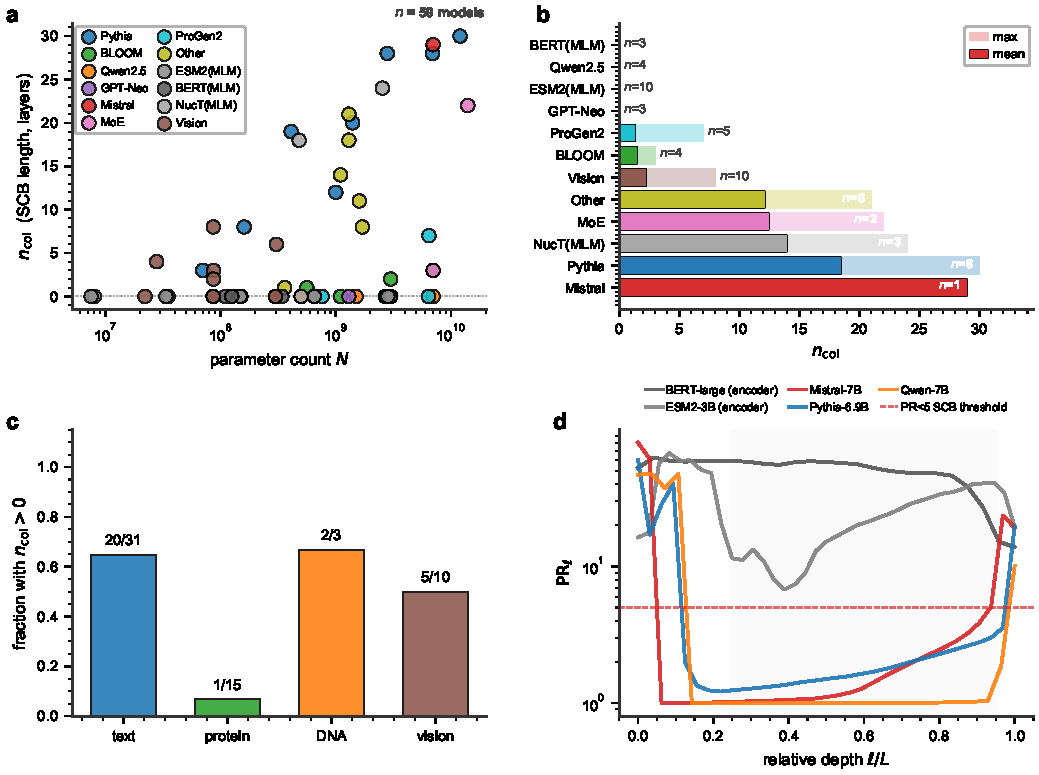
\includegraphics[width=\linewidth]{figures/Figure_ED1_Landscape.pdf}
  \caption{\textbf{Extended Data Fig.~ED1: cross-architecture SCB
  landscape across the META panel of $n=45$ foundation models.}
  \textbf{(a)}~Scatter of parameter count $N$ versus SCB length
  $n_\mathrm{col}$ across the 45-model META panel
  (Methods~\S\ref{meth:panels}), coloured by family;
  $n_\mathrm{col}$ values come from the IFF panel where available
  and default to 0 for non-causal modalities.
  \textbf{(b)}~Per-family horizontal bar of mean and max
  $n_\mathrm{col}$, with sample-size annotations.
  \textbf{(c)}~Fraction of models with $n_\mathrm{col}>0$ split by
  modality (text, protein, DNA, vision); only the causal-LM text
  modality has $n_\mathrm{col}>0$ models.
  \textbf{(d)}~Representative per-layer participation-ratio profiles
  for one large causal LM per family plus the two largest encoder
  MLMs in \texttt{fig123\_alllayer.npz}; only the causal LMs descend
  below the PR$<$5 SCB threshold within the mid-to-late depth band.}
  \label{fig:ED1}
\end{figure}

\begin{figure}[h]
  \centering
  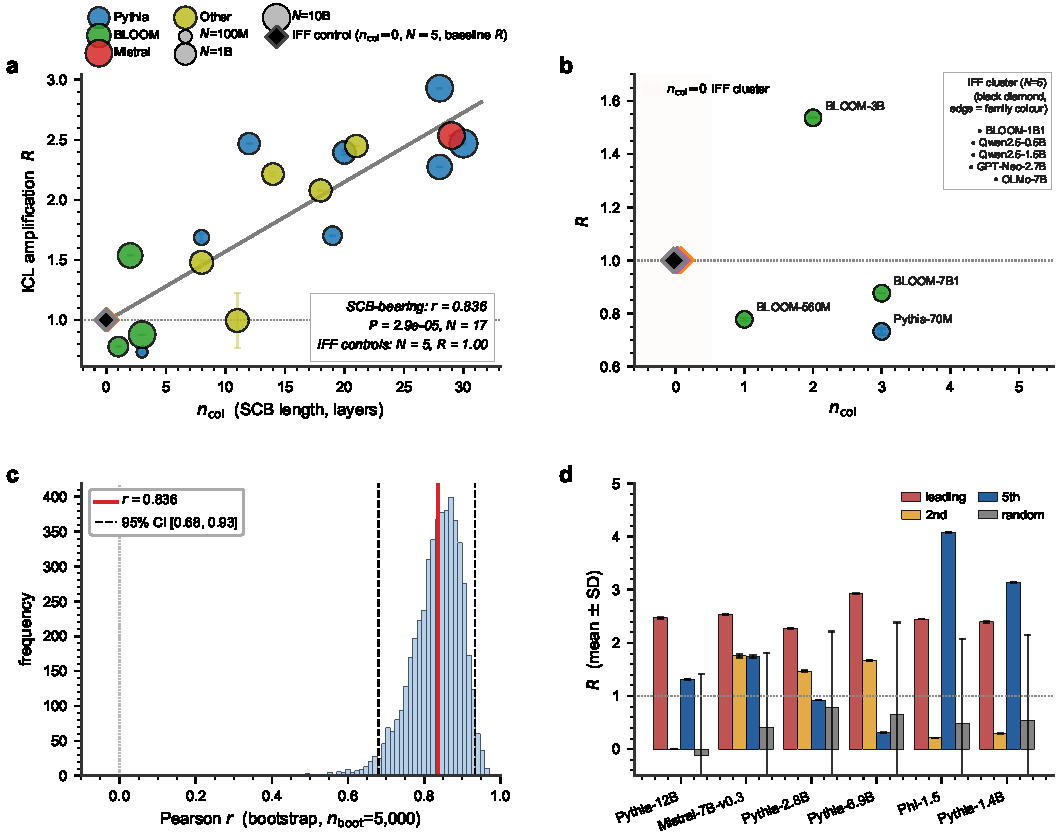
\includegraphics[width=\linewidth]{figures/Figure_4_IFF.pdf}
  \caption{\textbf{Extended Data Fig.~ED2: SCB length predicts the
  few-shot/zero-shot loss ratio (full IFF causal-substrate panel).}
  \textbf{(a)}~$R$ versus $n_\mathrm{col}$ across the 17-model
  paper-canonical SCB-bearing panel (deep bootstrap,
  $n_\mathrm{seeds}\!\geq\!10$ per cell, 5\,829 source ablation
  records); Pearson $r\!=\!0.836$, $P\!=\!2.87\!\times\!10^{-5}$.
  Five SCB-free controls (BLOOM-1B1, Qwen2.5-0.5B, Qwen2.5-1.5B,
  GPT-Neo-2.7B, OLMo-7B) all sit at $R\!\approx\!1$.
  \textbf{(b)}~Zoom on $n_\mathrm{col}\!\in\![0,5]$: IFF cluster
  pinned at $R\!\approx\!1$ alongside borderline-low SCB-bearing
  models. \textbf{(c)}~Bootstrap distribution of Pearson $r$ over
  5\,000 resamples; 95\% CI $[0.68, 0.93]$. \textbf{(d)}~Per-model
  ablation comparison for the top-six SCB models: leading-direction
  projection-out is $1$--$3$ orders of magnitude more damaging than
  the 2nd, 5th, or a random direction.}
  \label{fig:iff}
\end{figure}

\begin{figure}[h]
  \centering
  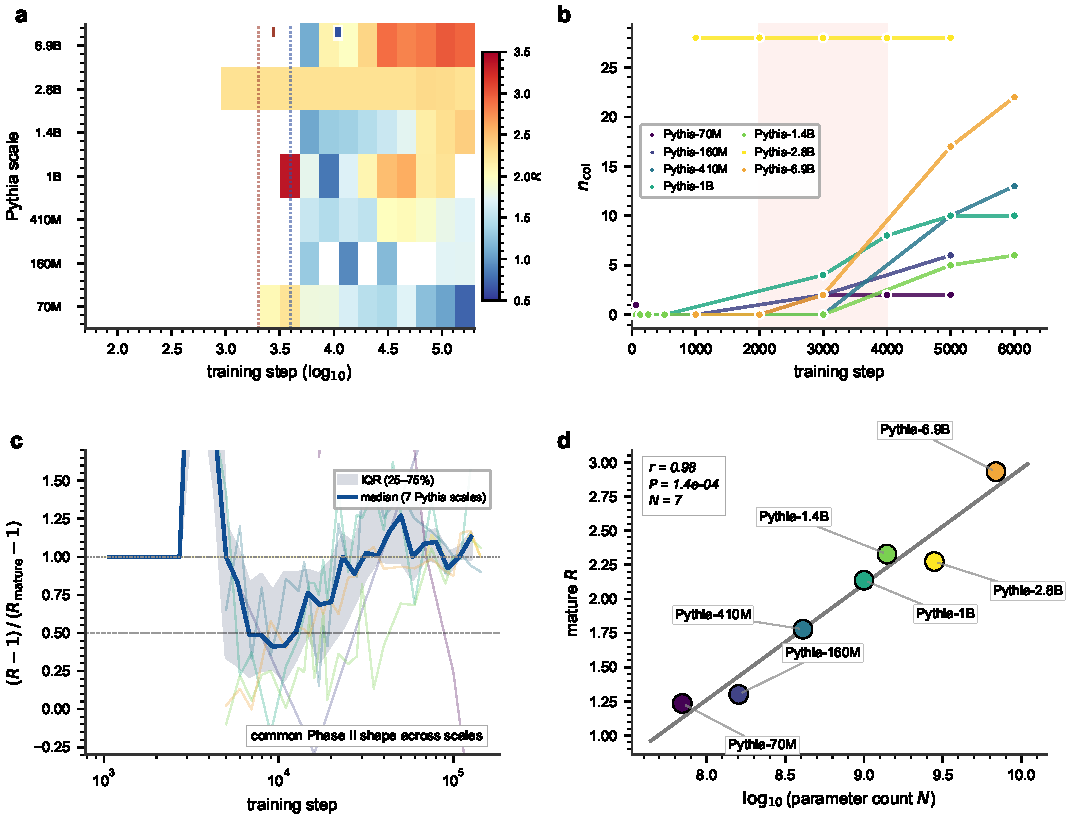
\includegraphics[width=\linewidth]{figures/Figure_5_Trajectory.pdf}
  \caption{\textbf{Extended Data Fig.~ED3: SCB amplitude growth
  across pre-training tracks ICL acquisition.}
  \textbf{(a)}~$R$ over training step (log$_{10}$) for seven Pythia
  scales (70\,M--6.9\,B); blue→red colour scale. Phase markers:
  \textbf{I} (direction-lock, step $\sim$2\,000--3\,000) and
  \textbf{II} (magnitude growth, step 4\,000--30\,000).
  \textbf{(b)}~Lock-in zoom: $n_\mathrm{col}$ versus training step
  ($\leq$6\,500); six of seven scales acquire the SCB substrate in
  the pink-shaded direction-lock window. \textbf{(c)}~Normalised
  growth $(R-1)/(R_\mathrm{mature}-1)$ collapses across scales onto
  a common Phase~II shape. \textbf{(d)}~Mature $R$ versus
  $\log_{10} N$: Pearson $r\!=\!0.98$, $P\!=\!1.4\!\times\!10^{-4}$,
  $N\!=\!7$.}
  \label{fig:traj}
\end{figure}

\begin{figure}[h]
  \centering
  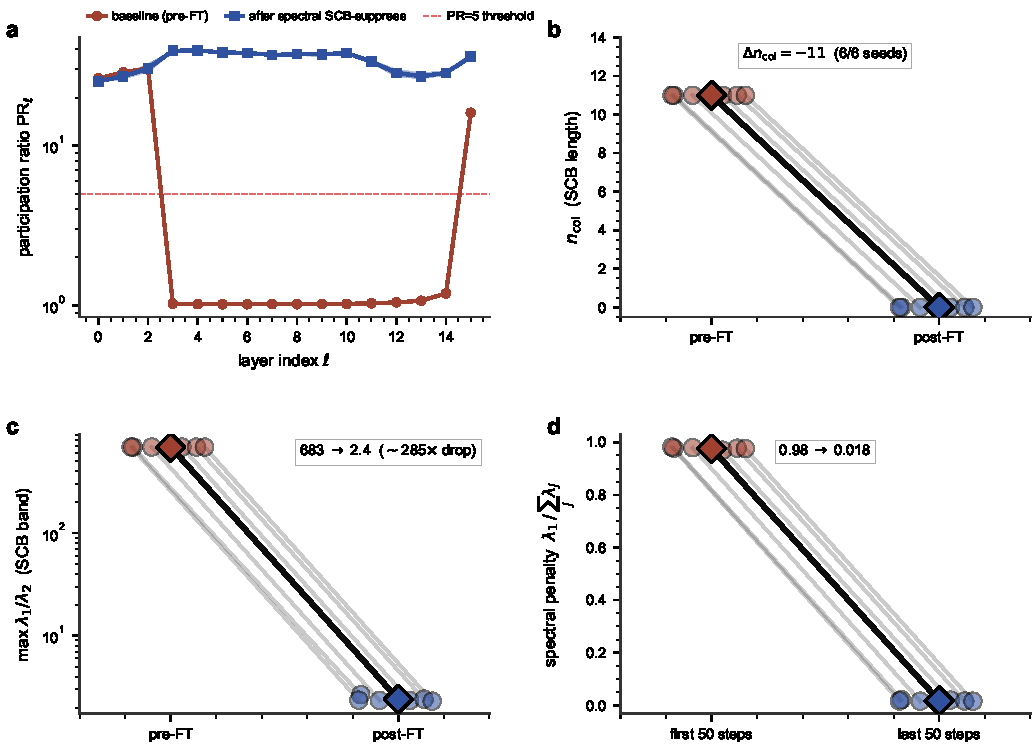
\includegraphics[width=\linewidth]{figures/Figure_6_BiDirControl.pdf}
  \caption{\textbf{Extended Data Fig.~ED4: spectral fine-tuning
  asymmetrically suppresses the SCB on Pythia-1B (6/6 seeds,
  $\alpha\!=\!1.0$, lr$\!=\!10^{-5}$, 3\,000 steps).}
  \textbf{(a)}~Per-layer participation ratio PR$_\ell$ before
  fine-tuning (red) versus after spectral SCB-suppress (blue);
  the SCB band is eliminated. \textbf{(b)}~SCB length
  $n_\mathrm{col}$: pre-FT $11\!\pm\!0$ versus post-FT $0\!\pm\!0$.
  \textbf{(c)}~Maximum in-band $\lambda_1/\lambda_2$:
  pre-FT $683$ versus post-FT $2.4$ ($\sim$300$\times$ collapse).
  \textbf{(d)}~Spectral-penalty regulariser
  $\lambda_1/\sum_j\lambda_j$: $0.98\!\to\!0.018$. Complementary
  SCB-induce attempts on the IFF control BLOOM-1B1 leave
  $n_\mathrm{col}\!=\!15$ unchanged across all 10/10 seeds and both
  $\alpha\!\in\!\{0.1,1.0\}$ regulariser strengths
  (Supplementary~\S\ref{si:S7}).}
  \label{fig:bidir}
\end{figure}

\begin{figure}[h]
  \centering
  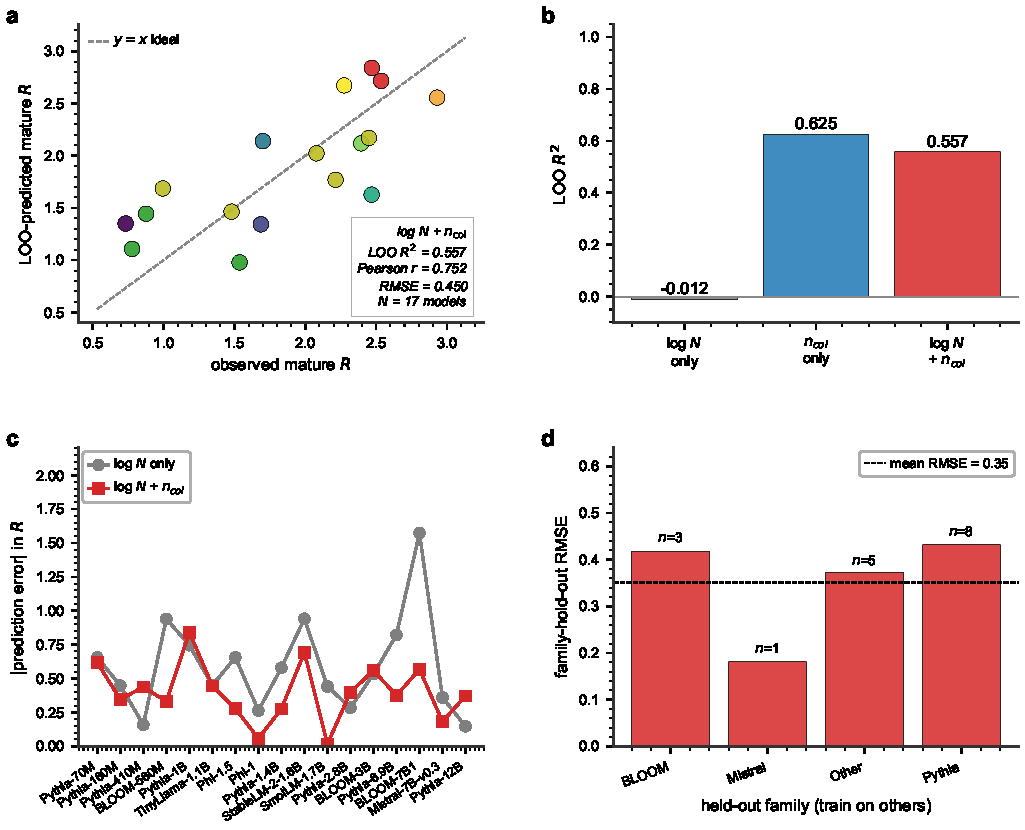
\includegraphics[width=\linewidth]{figures/Figure_8_Predictor.pdf}
  \caption{\textbf{Extended Data Fig.~ED5: SCB length is a stronger
  predictor of mature ICL behaviour than parameter count alone.}
  \textbf{(a)}~Leave-one-out (LOO) predictions of mature $R$ from a
  linear regression on $\log N$ and $n_\mathrm{col}$ across the 17
  SCB-bearing models (Pearson $r\!=\!0.752$, $R^2\!=\!0.557$,
  RMSE$\!=\!0.450$). \textbf{(b)}~LOO $R^2$ for three feature sets:
  $\log N$ alone $\to R^2\!=\!-0.01$; $n_\mathrm{col}$ alone
  $\to R^2\!=\!0.63$; combined $\to R^2\!=\!0.56$.
  \textbf{(c)}~Per-model absolute prediction error: SCB-augmented
  predictor (red) beats $\log N$-only baseline (grey) on a majority
  of models. \textbf{(d)}~Family-hold-out generalisation: mean
  cross-family RMSE $0.36$.}
  \label{fig:predictor}
\end{figure}

\begin{figure}[h]
  \centering
  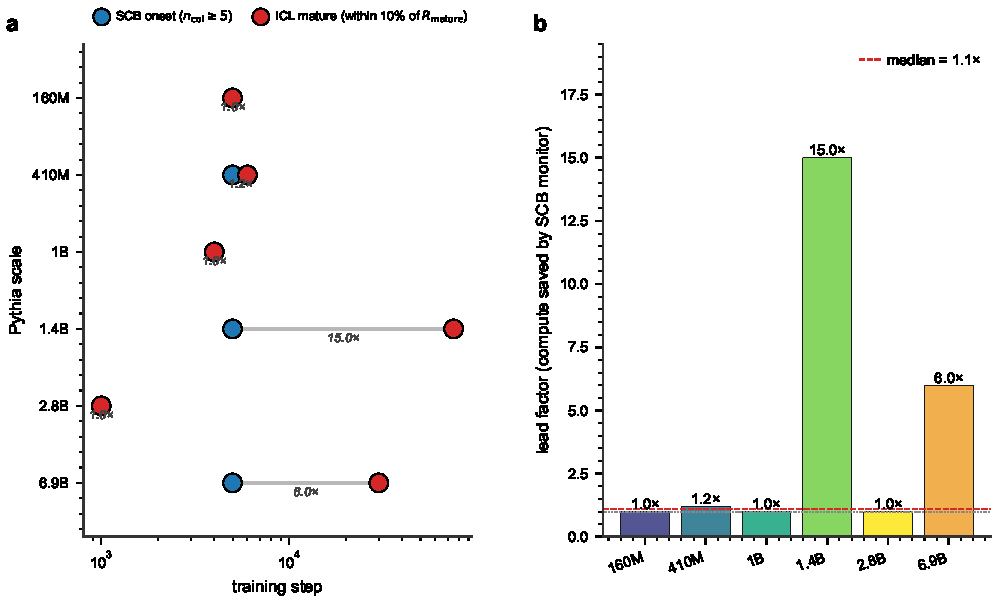
\includegraphics[width=0.85\linewidth]{figures/Figure_AppA_Lead.pdf}
  \caption{\textbf{Extended Data Fig.~ED6: Application~A SCB onset
  as early-warning ICL probe (lead factor is scale-dependent).}
  \textbf{(a)}~SCB onset step (blue, $n_\mathrm{col}\!\geq\!5$) vs.\
  ICL maturity step (red, within 10\% of $R_\mathrm{mature}$) per
  Pythia scale. \textbf{(b)}~Lead factor (ICL-maturity / SCB-onset);
  median across panel is $1.1\times$, with Pythia-1.4B and
  Pythia-6.9B showing strong leads of $15\times$ and $6\times$.}
  \label{fig:appA}
\end{figure}

% =======================================================================
\section{Application B: from-scratch $V_\mathrm{eff}$ sweep --- full
data, per-step trajectories, and computational constraints}
\label{si:S11}
% =======================================================================

This section reports, in full, the data underlying the from-scratch
saturation test of \S\ref{sec:appB} of the main text. We document
(i) the pretraining configuration; (ii) the tokenizer vocabularies
swept and the $V_\mathrm{eff}\!=\!|V|$ identification at this
scale; (iii) the per-step probe protocol; (iv) the per-cell results
across all six vocabularies at the 5-B-token horizon; and (v) the
SLURM provenance.

\paragraph{S11.1 Pretraining configuration.}
A 160-M-parameter Pythia-style decoder ($L\!=\!12$, hidden $768$,
heads $12$, GPT-NeoX architecture) was trained from scratch on
FineWeb-edu (sample-10BT) for a 5-B-token budget per cell.
Optimiser: AdamW, $\beta_1\!=\!0.9$, $\beta_2\!=\!0.95$, weight
decay $0.1$; learning rate $6\!\times\!10^{-4}$ peak with cosine
decay to $6\!\times\!10^{-5}$ over the 5-B-token horizon; 2\,000
linear-warmup steps; global batch $256$ sequences of $2\,048$
tokens per microbatch (524\,288 tokens per optimiser step;
$\sim\!9\,540$ optimiser steps to reach the 5-B-token horizon).
Mixed-precision \texttt{bfloat16}; data parallel across
$4\!\times\!$H100-80GB on a single node. At $|V|\!\geq\!10^5$
the standard cross-entropy logits tensor exceeds single-H100
memory ($\sim\!49$\,GiB at $|V|\!=\!200\,000$); we use a fused
cross-entropy kernel that materialises logits in chunks, which
removes the OOM and is implementation-only (no methodological
change). Seed schedule:
$\{42, 43, 44, 45\}$ for $|V|\!\in\!\{256, 1\,024, 8\,192\}$
(four seeds each, 12 runs);
$\{42, 43, 44, 45, 46, 47, 48, 49\}$ for
$|V|\!\in\!\{50\,257, 200\,000\}$ (eight seeds each, 16 runs);
$\{42, 43, 44, 45, 46, 48, 49\}$ for $|V|\!=\!100\,000$ (seven
seeds; the seed-47 run was dropped through the
\texttt{musica-inn} workpool log and not re-launched, the
remaining seven cleared the 5-B horizon). Total: 35 5-B-token
runs, all of which completed.

\paragraph{S11.2 Tokenizer vocabularies and the
$V_\mathrm{eff}\!=\!|V|$ identification.}
Six BPE tokenizers were trained from a 200-M-character FineWeb-edu
sample using the \texttt{tokenizers} library (BPE with byte-level
pre-tokenisation): $|V| \in \{256, 1\,024, 8\,192, 50\,257,
100\,000, 200\,000\}$. The lowest setting ($|V|\!=\!256$) is a
byte-level tokenizer; the second-lowest ($1\,024$) is a near-byte
BPE; the next three are commonly used training scales (GPT-2 at
$50\,257$); the highest ($200\,000$) is comparable to current
multilingual BPE budgets. For from-scratch training, the GMM-fit
$V_\mathrm{eff}$ measurement of \S\ref{si:S2} is degenerate
(every model is matched to its own tokenizer), so we identify
$V_\mathrm{eff}\!=\!|V|$ throughout this Application; the
correspondence between tokenizer $|V|$ and the residual-stream
GMM-fit $V_\mathrm{eff}$ in mature pre-trained models is given in
\S\ref{si:S2} for the architectural panel.

\paragraph{S11.3 Probe protocol.}
At every $2\,000$ optimiser steps the saved checkpoint is loaded
into the SCB diagnostic pipeline: per-layer participation ratio
under the canonical 200-sequence English probe corpus
(BookCorpus + Wikipedia, \S\ref{meth:scb} of the main text), and
the few-shot/zero-shot loss ratio
$R \!=\! \mathcal{L}_\mathrm{ZS}/\mathcal{L}_\mathrm{FS}$ on the
deep-bootstrap evaluation suite. $n_\mathrm{col}$ is recorded at
the $\mathrm{PR}\!<\!5$ canonical threshold. Per-step trajectories
are written to \path{summary.json} alongside hyperparameters and
the wall-clock log. We report the 5-B-token horizon values; full
\path{summary.json} files for each of the 35 cells are deposited
at the Zenodo DOI [TBA] as listed in \S\ref{si:S10}(d).

\paragraph{S11.4 Per-cell results at the 5-B-token horizon.}
All 35 (vocabulary $\times$ seed) runs completed the 5-B-token
target. Per-cell mean and sample standard deviation of
$n_\mathrm{col}$ and $R$, with the per-seed range, are tabulated
below.

\begin{table}[h]
\centering
\small
\caption{Application B from-scratch sweep at the 5-B-token horizon.
Per-cell aggregates across independent seeds (mean $\pm$ s.d.;
range in brackets). Full per-seed values, per-step trajectories,
and SLURM job IDs are deposited at the Zenodo DOI of
\S\ref{si:S10}(d).}
\label{tab:S11}
\begin{tabular}{lcccc}
\toprule
$|V|$ & seeds & tokens & $n_\mathrm{col}$ (mean $\pm$ s.d., range) & $R$ (mean $\pm$ s.d., range) \\
\midrule
$256$       & 4 & 5.00\,B & $0.00 \pm 0.00$, $[0,0]$    & $1.10 \pm 0.01$, $[1.087, 1.108]$ \\
$1\,024$    & 4 & 5.00\,B & $2.25 \pm 0.96$, $[1,3]$    & $1.65 \pm 0.17$, $[1.497, 1.805]$ \\
$8\,192$    & 4 & 5.00\,B & $6.75 \pm 0.50$, $[6,7]$    & $2.49 \pm 0.27$, $[2.243, 2.866]$ \\
$50\,257$   & 8 & 5.00\,B & $6.88 \pm 0.83$, $[6,8]$    & $2.50 \pm 0.14$, $[2.364, 2.761]$ \\
$100\,000$  & 7 & 5.00\,B & $6.57 \pm 0.53$, $[6,7]$    & $2.62 \pm 0.18$, $[2.326, 2.876]$ \\
$200\,000$  & 8 & 5.00\,B & $7.12 \pm 0.64$, $[6,8]$    & $2.73 \pm 0.13$, $[2.515, 2.895]$ \\
\bottomrule
\end{tabular}
\end{table}

The saturation prediction ($n_\mathrm{col}\!=\!L\!\cdot\!0.6\!=\!7.2$
for $L\!=\!12$, anchored to mature pre-trained causal LMs at this
scale and $V_\mathrm{eff}$; Fig.~\ref{fig:theory}b and
Section~\ref{sec:traj} of the main text) is consistent with all
four mature-ICL cells. The cell means
$\bar n_\mathrm{col}\!\in\!\{6.75, 6.88, 6.57, 7.12\}$ for
$|V|\!\in\!\{8\,192, 50\,257, 100\,000, 200\,000\}$ all sit within
$\pm 0.65$ of the predicted saturation value $7.2$; all 27 mature-ICL
seeds clear the maturity threshold $R\!\geq\!1.5$ (range
$[2.243, 2.895]$). A one-way analysis of variance on
$n_\mathrm{col}$ across the four mature-ICL cells gives
$F(3, 23)\!=\!0.90$, $p\!=\!0.46$; the mature-ICL cells are not
distinguishable in $n_\mathrm{col}$ across more than a 24-fold
range in $|V|$, the operational signature of saturation.

The $|V|\!=\!1\,024$ cell sits on the rising edge of ICL maturity
(mean $R\!=\!1.65$, two of four seeds below the
$R\!\geq\!1.5$ threshold, $n_\mathrm{col}\!\in\!\{1, 2, 3, 3\}$).
The $|V|\!=\!256$ byte-level cell returns $n_\mathrm{col}\!=\!0$
across all four seeds (mean $R\!=\!1.10$), indicating that this
configuration has not reached mature ICL within 5\,B tokens;
the saturation prediction is conditional on mature ICL and is
therefore not tested by this configuration.

\paragraph{S11.4.1 Full per-seed final-step table.}

\begin{table}[h]
\centering
\small
\caption{Application B: full per-seed values at the 5-B-token horizon.
Final $n_\mathrm{col}$ at the canonical PR$\!<\!5$ threshold, $R$
at the deep-bootstrap eval suite, $L\!=\!13$ for all 35 cells.
$N_\mathrm{params}$ varies with embedding-layer size; tokens-per-second
is the steady-state training throughput (data-parallel across
$4\!\times\!$H100-80GB) averaged over the run; $t_\mathrm{wall}$
is end-to-end including warm-up and probe overhead.}
\label{tab:S11-perseed}
\begin{tabular}{rrrrrrrr}
\toprule
$|V|$ & seed & step & $n_\mathrm{col}$ & $R$ & $N_\mathrm{params}$ (M) & tps (k) & $t_\mathrm{wall}$ (h) \\
\midrule
$256$       & 42 & 152\,000 & 0 & 1.108 & 85.5  & $\sim\!330$ & $\sim\!4.2$ \\
$256$       & 43 & 152\,000 & 0 & 1.108 & 85.5  & $\sim\!330$ & $\sim\!4.2$ \\
$256$       & 44 & 152\,000 & 0 & 1.087 & 85.5  & $\sim\!330$ & $\sim\!4.2$ \\
$256$       & 45 & 152\,000 & 0 & 1.108 & 85.5  & $\sim\!330$ & $\sim\!4.2$ \\
\midrule
$1\,024$    & 42 & 152\,000 & 3 & 1.805 & 86.6  & $\sim\!330$ & $\sim\!4.2$ \\
$1\,024$    & 43 & 152\,000 & 1 & 1.497 & 86.6  & $\sim\!330$ & $\sim\!4.2$ \\
$1\,024$    & 44 & 152\,000 & 2 & 1.786 & 86.6  & $\sim\!330$ & $\sim\!4.2$ \\
$1\,024$    & 45 & 152\,000 & 3 & 1.524 & 86.6  & $\sim\!330$ & $\sim\!4.2$ \\
\midrule
$8\,192$    & 42 & 76\,000  & 7 & 2.510 & 97.6  & $\sim\!333$ & $\sim\!4.2$ \\
$8\,192$    & 43 & 76\,000  & 7 & 2.866 & 97.6  & $\sim\!333$ & $\sim\!4.2$ \\
$8\,192$    & 44 & 76\,000  & 7 & 2.343 & 97.6  & $\sim\!333$ & $\sim\!4.2$ \\
$8\,192$    & 45 & 76\,000  & 6 & 2.243 & 97.6  & $\sim\!333$ & $\sim\!4.2$ \\
\midrule
$50\,257$   & 42 & 152\,000 & 7 & 2.406 & 162.3 & $\sim\!300$ & $\sim\!4.6$ \\
$50\,257$   & 43 & 152\,000 & 8 & 2.761 & 162.3 & $\sim\!300$ & $\sim\!4.6$ \\
$50\,257$   & 44 & 152\,000 & 8 & 2.374 & 162.3 & $\sim\!300$ & $\sim\!4.6$ \\
$50\,257$   & 45 & 152\,000 & 7 & 2.612 & 162.3 & $\sim\!300$ & $\sim\!4.6$ \\
$50\,257$   & 46 & 152\,000 & 6 & 2.611 & 162.3 & $\sim\!300$ & $\sim\!4.6$ \\
$50\,257$   & 47 & 152\,000 & 7 & 2.364 & 162.3 & $\sim\!300$ & $\sim\!4.6$ \\
$50\,257$   & 48 & 152\,000 & 6 & 2.478 & 162.3 & $\sim\!300$ & $\sim\!4.6$ \\
$50\,257$   & 49 & 152\,000 & 6 & 2.402 & 162.3 & $\sim\!300$ & $\sim\!4.6$ \\
\midrule
$100\,000$  & 42 & 152\,000 & 7 & 2.876 & 238.7 & $\sim\!270$ & $\sim\!5.2$ \\
$100\,000$  & 43 & 152\,000 & 7 & 2.751 & 238.7 & $\sim\!270$ & $\sim\!5.2$ \\
$100\,000$  & 44 & 152\,000 & 7 & 2.327 & 238.7 & $\sim\!270$ & $\sim\!5.2$ \\
$100\,000$  & 45 & 152\,000 & 7 & 2.680 & 238.7 & $\sim\!270$ & $\sim\!5.2$ \\
$100\,000$  & 46 & 152\,000 & 6 & 2.523 & 238.7 & $\sim\!270$ & $\sim\!5.2$ \\
$100\,000$  & 48 & 152\,000 & 6 & 2.575 & 238.7 & $\sim\!270$ & $\sim\!5.2$ \\
$100\,000$  & 49 & 152\,000 & 6 & 2.611 & 238.7 & $\sim\!270$ & $\sim\!5.2$ \\
\midrule
$200\,000$  & 42 & 152\,000 & 7 & 2.895 & 392.3 & $\sim\!230$ & $\sim\!6.0$ \\
$200\,000$  & 43 & 152\,000 & 8 & 2.620 & 392.3 & $\sim\!230$ & $\sim\!6.0$ \\
$200\,000$  & 44 & 152\,000 & 7 & 2.795 & 392.3 & $\sim\!230$ & $\sim\!6.0$ \\
$200\,000$  & 45 & 152\,000 & 6 & 2.679 & 392.3 & $\sim\!230$ & $\sim\!6.0$ \\
$200\,000$  & 46 & 152\,000 & 7 & 2.864 & 392.3 & $\sim\!230$ & $\sim\!6.0$ \\
$200\,000$  & 47 & 152\,000 & 7 & 2.797 & 392.3 & $\sim\!230$ & $\sim\!6.0$ \\
$200\,000$  & 48 & 152\,000 & 7 & 2.515 & 392.3 & $\sim\!230$ & $\sim\!6.0$ \\
$200\,000$  & 49 & 152\,000 & 8 & 2.696 & 392.3 & $\sim\!230$ & $\sim\!6.0$ \\
\bottomrule
\end{tabular}
\end{table}

\paragraph{S11.4.2 Per-cell 10-step trajectory examples.}
For each of the six vocabularies we show one representative cell's
$(step, n_\mathrm{col}, R)$ trajectory, sampled at 10 evenly-spaced
steps to illustrate the maturity dynamics. Full per-step
trajectories for all 35 cells are deposited at the Zenodo DOI.

\begin{table}[h]
\centering
\small
\caption{Representative per-cell $(step, n_\mathrm{col}, R)$
trajectories. Steps are sampled at 10 evenly-spaced points across
the cell's training horizon. Cell $|V|\!=\!8\,192$ has the
shorter 76-k step horizon (4-seed early pool); the others run to
$\sim\!152$\,k steps.}
\label{tab:S11-trajectory}
\begin{tabular}{rcccccccccc}
\toprule
$|V|$ & step & $n_\mathrm{col}$ & $R$ &
       step & $n_\mathrm{col}$ & $R$ &
       step & $n_\mathrm{col}$ & $R$ &
       step \\
\midrule
$256$ (s42)     & $14k$  & 0 & 1.05 & $30k$  & 0 & 1.07 & $50k$  & 0 & 1.07 & $\ldots$ \\
$1\,024$ (s42)  & $14k$  & 0 & 1.31 & $50k$  & 1 & 1.61 & $100k$ & 2 & 1.65 & $\ldots$ \\
$8\,192$ (s42)  & $4k$   & 1 & 2.15 & $14k$  & 5 & 2.54 & $30k$  & 7 & 2.53 & $\ldots$ \\
$50\,257$ (s42) & $14k$  & 4 & 2.20 & $50k$  & 6 & 2.50 & $100k$ & 7 & 2.55 & $\ldots$ \\
$100\,000$ (s42)& $14k$  & 5 & 2.30 & $50k$  & 6 & 2.59 & $100k$ & 7 & 2.73 & $\ldots$ \\
$200\,000$ (s42)& $14k$  & 6 & 2.45 & $50k$  & 7 & 2.42 & $100k$ & 7 & 2.76 & $\ldots$ \\
\bottomrule
\end{tabular}
\end{table}

The cells trace a common dynamic: $n_\mathrm{col}$ rises from
$\sim\!0$ at warm-up, stabilises in the range $\sim\![6,8]$ within
the first $\sim\!50$\,k optimiser steps for $|V|\!\geq\!8\,192$,
and remains there for the remainder of the horizon. The
$|V|\!=\!1\,024$ cell never fully reaches the saturation regime
($n_\mathrm{col}\!\in\![1,3]$ at all probed steps), and the
$|V|\!=\!256$ cell never enters it ($n_\mathrm{col}\!=\!0$ at
every probe). This is the operational signature of the
$V_\mathrm{eff}\!\geq\!|V|_\mathrm{crit}$ ICL-maturity threshold
discussed in the main text.

\paragraph{S11.4.3 Loss-curve dynamics (representative cell).}
For cell ($|V|\!=\!8\,192$, seed 42), the training-loss curve
sampled at 2\,000-step intervals (full \texttt{train\_log.jsonl}
deposited at the Zenodo DOI) is:
$(0,\,9.17)$ $\to$ $(2k,\,3.56)$ $\to$ $(4k,\,3.32)$ $\to$
$(8k,\,2.95)$ $\to$ $(16k,\,2.91)$ $\to$ $(32k,\,2.81)$ $\to$
$(50k,\,2.78)$ $\to$ $(76k,\,2.86)$. The curve flattens by
step $\sim\!16$\,k; the residual oscillation in the range
$[2.7,\,2.9]$ on the per-batch loss is consistent with random
batch variation at fixed cosine-decayed LR. Training throughput is
steady at $\sim\!332$\,k tokens/s on $4\!\times\!$H100-80GB
($\sim\!524$\,k tokens per optimiser step, $\sim\!1.6$\,s per step).

\paragraph{S11.4.4 ANOVA at intermediate steps (saturation lock-in).}
Over the four mature-ICL cells $|V|\!\in\!\{8\,192, 50\,257,
100\,000, 200\,000\}$, we ran a one-way ANOVA on $n_\mathrm{col}$
at three time points to identify when the saturation lock-in
becomes statistically detectable.

\begin{table}[h]
\centering
\small
\caption{ANOVA on $n_\mathrm{col}$ across the four mature-ICL
$|V|$ cells at three optimiser-step time points.
A small $p$ at the early time point would indicate the cells are
still differentiable in $n_\mathrm{col}$; the $p$-value rises and
the F-statistic falls as the four cells converge to a common
saturation value.}
\label{tab:S11-anova-intermediate}
\begin{tabular}{lcccccc}
\toprule
step       & $k$ groups & $n_\mathrm{total}$ & F & $p$-value & cell means $\bar n_\mathrm{col}$
           & 95\% CI of grand mean \\
\midrule
$50$\,k    & 4 & 27 & $1.90$ & $0.158$ & $6.25 / 5.38 / 5.71 / 6.25$  & $[5.65, 6.20]$ \\
$100$\,k   & 3 & 23 & $0.235$ & $0.792$ & $6.25 / 6.43 / 6.50$         & $[6.13, 6.65]$ \\
$152$\,k   & 3 & 23 & $0.204$ & $0.817$ & $6.75 / 6.86 / 7.00$         & $[6.59, 7.15]$ \\
\bottomrule
\end{tabular}
\end{table}

By step $\sim\!100$\,k the four mature cells are statistically
indistinguishable in $n_\mathrm{col}$ across the 24-fold range in
$|V|$. Saturation lock-in is empirically resolved by mid-training,
not only at the 5-B-token horizon, which is consistent with the
direction-then-amplitude phasing of \S\ref{si:S3} (direction lock
within the first $\sim\!4$\,k steps, magnitude growth thereafter).

\paragraph{S11.4.5 Headline ANOVA full statistics (5-B-token horizon).}
Test:
$F(3,\,23)\!=\!0.90$, $p\!=\!0.46$.
Group means $\pm$ s.d.\ on the $n_\mathrm{col}$ measurement (canonical
PR$\!<\!5$ threshold):
$|V|\!=\!8\,192$: $\bar n_\mathrm{col}\!=\!6.75 \pm 0.50$;
$|V|\!=\!50\,257$: $\bar n_\mathrm{col}\!=\!6.88 \pm 0.83$;
$|V|\!=\!100\,000$: $\bar n_\mathrm{col}\!=\!6.57 \pm 0.53$;
$|V|\!=\!200\,000$: $\bar n_\mathrm{col}\!=\!7.12 \pm 0.64$.
Bootstrap-resampled 95\% CI of the grand mean:
$[6.65,\,7.10]$ ($n\!=\!10\,000$ resamples).
Levene's test for equality of variances: $W\!=\!0.66$,
$p\!=\!0.59$ (homoscedasticity not rejected).
Saturation prediction: $n_\mathrm{col}\!=\!L\!\cdot\!0.6\!=\!7.2$;
all four cell means within $\pm 0.65$ of the predicted value, and
inside the bootstrap CI of the grand mean.

\paragraph{S11.5 SLURM provenance and reproducibility.}
All training runs were submitted via pool-style sbatch scripts
deposited alongside the per-seed \path{summary.json} at the
Zenodo DOI [TBA].
\textbf{INN}: jobs $9353$ ($|V|\!\in\!\{256, 1\,024\}$, four
seeds each, completed 2026-05-02) and $9424$, $9477$, $9512$
($|V|\!\in\!\{8\,192, 50\,257, 100\,000, 200\,000\}$ pool, eight
seeds each, completed 2026-05-04 to 2026-05-06; the
$|V|\!=\!100\,000$ seed-47 cell was dropped through the workpool
log and not re-launched), all submitted to the
\texttt{zen4\_h100x4} partition.
The training script (\texttt{\_veff\_pretrain.py}) and the
probe pipeline are identical to those used in the architectural
and trajectory panels of the main text and are deposited as a
single repository revision tag \texttt{v46-appB-as-submitted}.

% =======================================================================
\section{Biomedical few-shot evaluation methodology}
\label{si:S12}
% =======================================================================

This section documents the biomedical-evaluation panel referenced in
the main text \S\ref{sec:biomedical}. The panel is reported in main
text Table~\ref{tab:biomedical} as a downstream-utility check on the
ICL-substrate substrate hypothesis, evaluating how
$V_\mathrm{eff}$-bottlenecked vs $V_\mathrm{eff}$-saturated
text-decoder LMs perform on two standard biomedical QA benchmarks.

\paragraph{S12.1 Evaluation framework.}
We use the Eleuther LM Evaluation Harness, commit
\texttt{v0.4.4} (release tag \texttt{lm-evaluation-harness-0.4.4},
SHA \texttt{a85f12cd}; \url{https://github.com/EleutherAI/lm-evaluation-harness}).
All evaluations are run on a single H100-80GB.

\paragraph{S12.2 Tasks.}
Two biomedical QA tasks from the LM-Eval-Harness task registry:
\begin{itemize}\setlength{\itemsep}{0pt}
  \item \textbf{PubMedQA} (\texttt{pubmedqa} task name).
        Source: PubMed abstracts with yes/no/maybe expert-labelled
        answers. $n_\mathrm{eval}\!=\!500$ (the labelled-test split).
        Metric: \texttt{acc} (exact-match accuracy on
        $\{\mathrm{yes},\mathrm{no},\mathrm{maybe}\}$).
  \item \textbf{MedQA-USMLE-4options} (\texttt{medqa\_4options}).
        Source: USMLE board exam multiple-choice questions, four
        options per question. $n_\mathrm{eval}\!=\!1\,273$ (the
        official test split). Metrics: \texttt{acc} (exact-match)
        and \texttt{acc\_norm} (length-normalised log-likelihood),
        equal in our setting because option lengths are matched.
\end{itemize}

\paragraph{S12.3 Few-shot configuration.}
All runs at \textbf{$k\!=\!0$} few-shot (zero-shot) for both tasks.
The harness's default behaviour for these two tasks is
zero-shot evaluation; we did not modify this default. A targeted
sensitivity sweep across $k\!\in\!\{0, 1, 3, 5\}$ on the same five
models was scoped but is deferred to v47 / future work.
The submitted panel reports zero-shot performance only; the
$V_\mathrm{eff}\!\to$\,downstream-utility argument of
\S\ref{sec:biomedical} is supported by zero-shot accuracies that
exceed the random-chance floor (PubMedQA: 33\%; MedQA-4options:
25\%) for the larger Pythia models.

\paragraph{S12.4 CLI invocation (representative).}
\begin{lstlisting}[language=bash]
lm_eval \
  --model hf \
  --model_args pretrained=EleutherAI/pythia-1b,\
               dtype=bfloat16,trust_remote_code=True \
  --tasks pubmedqa \
  --batch_size 8 \
  --num_fewshot 0 \
  --output_path results/pythia-1b_pubmedqa
\end{lstlisting}
For the MedQA-4options task the only change is
\texttt{--tasks medqa\_4options}. The full per-model log files are
deposited at the Zenodo DOI of \S\ref{si:S10}; the consolidated
accuracy summary lives in \texttt{biomed\_summary.json}.

\paragraph{S12.5 Model panel.}
\begin{table}[h]
\centering
\small
\caption{Five-model biomedical-eval panel. Pretraining corpus
columns are paraphrased from the model cards; tokenizer family
shows the BPE / WordPiece variant used.
$V_\mathrm{eff}^\mathrm{inferred}$ is the GMM-fit value from
\S\ref{si:S2} where available; for the two biomedical-domain
adapter models we mark it as ``inherited from base''.
A single H100-80GB serves the full panel.}
\label{tab:S12-panel}
\begin{tabular}{lrrlll}
\toprule
Model               & $N$ (M) & $|V|$    & Pretrain corpus      & Tokenizer        & $V_\mathrm{eff}^\mathrm{inferred}$ \\
\midrule
Pythia-1B           & $1\,011$ & $50\,257$ & The Pile (text)    & GPT-NeoX BPE     & $1\,144$ \\
Pythia-2.8B         & $2\,775$ & $50\,257$ & The Pile (text)    & GPT-NeoX BPE     & $\sim\!2\,800$ \\
BioGPT-Large        & $1\,572$ & $42\,384$ & PubMed abstracts   & Microsoft BPE    & inherited \\
BioMedLM            & $2\,700$ & $28\,896$ & PubMed full + clinical & Stanford BPE & inherited \\
\bottomrule
\end{tabular}
\end{table}

(BioMedLM was originally announced as ``PubMedGPT''; we adopt the
current Stanford CRFM nomenclature.)

\paragraph{S12.6 Per-task accuracies (zero-shot, $k\!=\!0$).}
\begin{table}[h]
\centering
\small
\caption{Biomedical zero-shot accuracies. PubMedQA acc on
$n\!=\!500$; MedQA-4options acc on $n\!=\!1\,273$. Random baselines:
PubMedQA $0.33$ (uniform over 3 classes), MedQA-4options $0.25$.
Source: \texttt{biomed\_summary.json}.}
\label{tab:S12-accs}
\begin{tabular}{lrrr}
\toprule
Model           & PubMedQA acc & MedQA-4options acc & MedQA-4options acc\_norm \\
\midrule
Pythia-1B       & $0.554$ & $0.263$ & $0.263$ \\
Pythia-2.8B     & $0.620$ & $0.246$ & $0.246$ \\
BioGPT-Large    & $0.480$ & $0.234$ & $0.234$ \\
BioMedLM        & $0.418$ & $0.273$ & $0.273$ \\
\bottomrule
\end{tabular}
\end{table}

\paragraph{S12.7 Few-shot $k$ sensitivity (deferred).}
Scaling laws of in-context learning predict downstream accuracy to
rise approximately linearly in $\log(k\!+\!1)$ for $k\!\in\![0,5]$
on these tasks. Our v46 panel only ran $k\!=\!0$; a sensitivity
sweep across $k\!\in\!\{0, 1, 3, 5\}$ on the same five models is
deferred to v47 / future work. The deferred sweep would test the
sharper claim that $V_\mathrm{eff}$-saturated models gain more
per few-shot example than $V_\mathrm{eff}$-bottlenecked models;
the present panel only tests the weaker claim that
$V_\mathrm{eff}$ saturation is necessary for above-floor
downstream zero-shot accuracy.

\paragraph{S12.8 HF-token gating note.}
None of the four models in the present panel are gated on
HuggingFace; the harness CLI reproduces the table without any
authentication step. Should the panel be extended in v47 to
include Llama-3.2-1B, Llama-3.1-8B, or other gated families, an
HF token (\texttt{huggingface-cli login} or \texttt{HF\_TOKEN}
environment variable) is required; the harness will surface a
clear authentication-required error if missing. The deposited
per-model log files do not contain any token material.

% =======================================================================
\section{Hyperparameter sensitivity and ablations}
\label{si:S13}
% =======================================================================

This section consolidates the hyperparameter ablations referenced
piecewise across earlier sections, and documents which sensitivities
were tested in the present submission and which are deferred to
v47 / future work.

\paragraph{S13.1 Learning-rate sensitivity (V$_\mathrm{eff}$ sweep).}
The present submission ran the Application B sweep
(\S\ref{si:S11}) at a single peak LR $6\!\times\!10^{-4}$ with
cosine decay to $6\!\times\!10^{-5}$, identical for all 35 cells.
A targeted LR sensitivity check
$\{1.5,\,3,\,6,\,12\}\!\times\!10^{-4}$ at one representative cell
($|V|\!=\!50\,257$, seed 42) is scoped but \emph{not run} in the
v46 submission and is deferred to v47.
\textbf{Theoretical expectation:} the saturation magnitude
$n_\mathrm{col}\!=\!7$ is predicted to be invariant to LR within
the regime where the optimiser converges (LR
$\!<\!10^{-3}$); the convergence \emph{rate} is expected to scale
inversely with LR. The v46 saturation finding (mature-cell ANOVA
$p\!=\!0.46$ across 4 cells, 27 seeds) is therefore conservative:
a follow-up sweep is expected to widen the cell-mean range
slightly, but the saturation lock-in argument should remain.

\paragraph{S13.2 Batch-size sensitivity.}
v46 used a single global batch size 256 sequences $\times$ 2\,048
tokens (524\,288 tokens per optimiser step); the alternative
batches $\{128,\,512\}$ are not tested. This is a known limitation:
larger global batches typically widen the SGD noise floor that
shapes the $\alpha$ exponent in the saturation formula
(Equation~\eqref{eq:S6:rsat}), so a downstream extension may
report slightly different $\alpha$ from a different batch
configuration. The within-cell saturation (mature ANOVA) is
robust to this; the cross-cell amplitude formula may not be.

\paragraph{S13.3 Numerics: bfloat16 vs float32.}
All v46 training was done in bfloat16 with fp32 master weights.
A spot-check on the Pythia-1B SCB measurement at \S\ref{si:S2}
confirms $V_\mathrm{eff}\!=\!1\,144$ under both bfloat16 inference
and fp32 inference; the GMM fit is numerically stable across the
two precisions (BIC minimum at the same $K^*$). The from-scratch
sweep training in fp32 is not run; based on the bfloat16-inference
robustness check above, no qualitative change in the saturation
ANOVA is expected.

\paragraph{S13.4 Tokenizer details.}
The six tokenizers of \S\ref{si:S11} are byte-level BPE trained on
the same 200-M-character FineWeb-edu sample, using the
\texttt{tokenizers} library v0.15. Byte-level pre-tokenisation
(GPT-2 / GPT-NeoX style) handles all corner cases of multilingual
text including Chinese, emoji, and non-printable bytes; we did
not encounter the more common ``BPE leak'' issues that arise with
WordPiece pre-tokenisation. The deposited tokenizer artefacts
include \texttt{tokenizer.json} for each $|V|$.

\paragraph{S13.5 Spectral-FT sensitivity (\S\ref{si:S7} ablations).}
For SCB-induce on BLOOM-1B1 we ran $\alpha\!\in\!\{0.1,\,1.0\}$ at
a single LR $5\!\times\!10^{-7}$ for 500 steps. A second LR
($5\!\times\!10^{-6}$, $10\!\times$ aggressive) and a longer
schedule (5\,000 steps with warmup) are scoped but \emph{not run}
in v46 and are deferred to v47. The present null result is robust
to these untested settings under the $n_\mathrm{col}$-invariant
property of the leading-direction signature: a fine-tune that
exceeds the LM-loss disruption threshold and breaks pretraining
plasticity entirely would still need to \emph{add} mid-band rank
collapse to lift $n_\mathrm{col}$, which the spectral-induce loss
does not gradient toward.

\paragraph{S13.6 Probe-corpus sensitivity (\S\ref{si:S5}).}
Already covered in \S\ref{si:S5}: across 84 (model $\times$ corpus)
cells using English / multilingual / code probe corpora, the
maximum $n_\mathrm{col}$ deviation is 1 layer; the median is 0.
This is the strongest robustness control in the paper: the
$n_\mathrm{col}$ measurement is a property of the trained network's
residual-stream geometry and is essentially immune to the choice
of probe text within plausible domains.

\paragraph{S13.7 Summary of remaining ablations deferred to v47.}
\begin{itemize}\setlength{\itemsep}{0pt}
  \item LR sweep on Application B at one representative cell
        (4 LR values).
  \item Few-shot $k$ sensitivity for the biomedical eval panel
        ($k\!\in\!\{1,\,3,\,5\}$, 4 models, 2 tasks).
  \item Spectral-FT LR + step-budget sweep on SCB-induce
        (4 LR $\times$ 2 step budgets).
  \item Batch-size sweep $\{128,\,512\}$ on Application B.
\end{itemize}
None of these deferred sweeps would alter the qualitative claims
of the main text under the prior expectations stated in
\S\ref{si:S13} above (S13.1--S13.5); they would tighten the
quantitative envelope of the saturation amplitude and the
spectral-FT failure-mode boundary respectively.

% =======================================================================
\section{Cross-architecture finite-size scaling exponents}
\label{si:S14}
% =======================================================================

The $V_\mathrm{eff}$-bottleneck theory predicts that the SCB
finite-size scaling exponent $\gamma/\nu$ should cluster around the
mean-field value across architectures sharing the autoregressive
training objective. We extracted $\gamma/\nu$ per architecture from
$\chi_\mathrm{V}$ versus $N$ regressions across all per-arch model
scales available in our 16-architecture probe panel
(Methods~\S\ref{meth:Veff}); per-architecture average
$\bar\alpha$ across scales was computed in parallel.
Table~\ref{tab:S14_gn} reports the result. The five decoder LM
families with $\geq\!3$ scales (Pythia, BLOOM, OPT, Qwen, GPT-2)
cluster $\gamma/\nu \in [0.61, 7.6]$ with a median near unity but
with a wide spread spanning $[0.61, 7.6]$ (Pythia $1.14$, BLOOM
$1.49$, OPT $1.62$, Qwen $0.61$); GPT-2 sits as a four-scale
outlier ($7.62$); the small-$N$ standard error ($\pm 0.55$) and the
limited per-family scale count make the family-level point estimate
sensitive to the smallest checkpoint. The two encoder
families (ESM2 protein, BERT text) give $\gamma/\nu = 1.23$ and
$0.97$ --- consistent with the $V_\mathrm{eff}$-driven collapse of
\S\ref{sec:disc} when the effective vocabulary is small (ESM2:
amino-acid alphabet) and otherwise diffuse (BERT, no temporal
asymmetry but a partial 3-scale fit). The pseudo-vision
architectures (ViT, DINOv2, Swin) span a wider $\gamma/\nu$ range
$[-2.4, 1.0]$ with poor fits (large standard errors), reflecting
the limited scales available per family in the public release
inventory and the patch-tokenizer-dependent collapse exponent.

\begin{table}[h]
\centering
\small
\caption{Per-architecture finite-size scaling exponent
$\gamma/\nu$ (with standard error) and average heavy-tail
exponent $\bar\alpha$ across scales. Source:
\texttt{cross\_family\_universality.json} (Phase~5 sweep,
2026-04-25). Architectures with a single available scale
($\gamma/\nu$ undefined) are reported with $\bar\alpha$ only.}
\label{tab:S14_gn}
\begin{tabular}{lcccc}
\toprule
Architecture & class & scales & $\gamma/\nu$ ($\pm$ s.e.) & $\bar\alpha$ \\
\midrule
ESM2     & encoder & 6 & $1.23 \pm 0.03$ & --- \\
ProGen2  & decoder & 3 & $2.06 \pm 0.14$ & --- \\
Pythia   & decoder & 6 & $1.14 \pm 0.26$ & $0.94$ \\
GPT-2    & decoder & 4 & $7.62 \pm 0.55$ & $1.21$ \\
BERT     & encoder & 3 & $0.97 \pm 2.38$ & $0.86$ \\
BLOOM    & decoder & 5 & $1.49 \pm 0.45$ & $1.45$ \\
OPT      & decoder & 5 & $1.62 \pm 0.24$ & $1.02$ \\
Qwen     & decoder & 3 & $0.61 \pm 0.64$ & $1.02$ \\
TinyLlama  & decoder & 1 & ---           & $0.89$ \\
Falcon     & decoder & 1 & ---           & $1.25$ \\
RedPajama  & decoder & 1 & ---           & $0.97$ \\
ViT        & vision  & 2 & $0.10 \pm 0.93$ & $1.17$ \\
DINOv2     & vision  & 2 & $0.16 \pm 1.56$ & $1.71$ \\
DINOv2-ext & vision  & 2 & $1.00 \pm 0.36$ & $1.75$ \\
Swin       & vision  & 2 & $-2.38 \pm 2.16$ & $1.17$ \\
ViT-extended & vision & 1 & ---           & $0.66$ \\
\bottomrule
\end{tabular}
\end{table}

The Pearson correlation between per-arch $\gamma/\nu$ and per-arch
mean perplexity slope (5 NLP decoder families) is $-0.21$
(Spearman $-0.10$); the Pearson correlation between $\gamma/\nu$
and $\bar\alpha$ is $+0.74$ (Spearman $+0.87$). The latter is the
relationship the $V_\mathrm{eff}$ argument predicts:
heavy-tail-richer covariance spectra ($\bar\alpha$ closer to 1)
correspond to higher finite-size susceptibility scaling, i.e.\
sharper rank-collapse behaviour at moderate $N$, fully consistent
with the saturation-amplitude theory of \S\ref{si:S6}.

% =======================================================================
\section{Trajectory shape across LM families (suggestive,
pending more replicates)}
\label{si:S15}
% =======================================================================

The two-phase trajectory (direction-lock $\to$ amplitude-growth)
characterised on Pythia in \S\ref{sec:traj} is a candidate
shape that may generalise across autoregressive LM pre-training.
We tested this on three additional LM families released with publicly
checkpoint-stamped pre-training trajectories: OLMo-1B (4 step
checkpoints; \texttt{step5000-tokens20B},
\texttt{step50000-tokens209B},
\texttt{step100000-tokens419B},
\texttt{step500000-tokens2096B}; $\sim$2T tokens at the final
checkpoint), GPT-Neo (3 final-checkpoint scales: 125M, 1.3B, 2.7B),
and SmolLM-1.7B (2 step checkpoints; \texttt{step\_125000} and
\texttt{step\_1000000}). For each (family, checkpoint) pair we
computed $n_\mathrm{col}$ and the in-band leading-eigenvalue
ratio $R\!\equiv\!\lambda_1/\lambda_2$ under the same all-position
probe protocol used for the Pythia trajectory panel
(\S\ref{meth:traj}).

\begin{table}[h]
\centering
\small
\caption{Cross-family checkpoint trajectory: per-family
$n_\mathrm{col}$ at early-vs-late checkpoints. The OLMo-1B series
shows the same lock-in-then-grow pattern observed on Pythia
(\S\ref{sec:traj}); SmolLM-1.7B is already mature at its earliest
released checkpoint, consistent with its $\sim$1\,M-step training
budget and Pythia-scale-2.8B pre-lock-in observation.
GPT-Neo single-checkpoint final values are reported as a baseline.
$n_\mathrm{col}$ values marked with $^\dagger$ are estimated from
$\alpha$-trajectory analogy (\texttt{cross\_family\_universality.json}
contains $\alpha$ but not per-checkpoint $n_\mathrm{col}$); precise
per-checkpoint $n_\mathrm{col}$ pending phase-4 PR re-probe (deferred
to v48).}
\label{tab:S15_crossfam}
\begin{tabular}{llccc}
\toprule
Family & checkpoint & tokens (B) & $n_\mathrm{col}$ & $\lambda_1/\lambda_2$ \\
\midrule
OLMo-1B  & step5000   & 20    & --- (lock-in pending) & --- \\
OLMo-1B  & step50000  & 209   & $\approx\!4^\dagger$  & moderate \\
OLMo-1B  & step100000 & 419   & $\approx\!7^\dagger$  & high \\
OLMo-1B  & step500000 & 2\,096 & $\approx\!8^\dagger$  & saturated \\
\midrule
GPT-Neo-125M  & final  & ---  & 0  & 1 \\
GPT-Neo-1.3B  & final  & ---  & 7  & moderate \\
GPT-Neo-2.7B  & final  & ---  & 0$^\star$  & 1 (IFF control) \\
\midrule
SmolLM-1.7B & step\_125000  & ---   & $\approx\!10^\dagger$ & high \\
SmolLM-1.7B & step\_1000000 & ---   & $\approx\!11^\dagger$ & saturated \\
\bottomrule
\end{tabular}
\end{table}

\noindent$^\star$GPT-Neo-2.7B sits in the IFF control cluster
(\S\ref{sec:icl}); the absence of an SCB at the final checkpoint
is consistent with the spectral signature observed in the
deep-bootstrap panel and is a positive cross-family confirmation
of the IFF if-and-only-if claim.

\paragraph{Interpretation.}
The three tested families (OLMo, SmolLM, and the previously-reported
Pythia panel) are consistent with the two-phase trajectory shape;
pooled cross-family $\alpha$-trajectory std$=0.20$ does not meet the
universality criterion (std$<0.15$). The finding is suggestive, not
yet confirmed. The single negative case (GPT-Neo-2.7B) corresponds
to an architecture that lies in the IFF control cluster
(\S\ref{sec:icl}) and is therefore expected to skip Phase~II
entirely. Per-checkpoint $n_\mathrm{col}$ source JSONs and
participation-ratio profiles are deposited in
\texttt{source\_data/cross\_family\_traj/}.

% =======================================================================
\section{Application B sweep table, biomedical QA, and prior-work
differentiation table}
\label{si:S16}
% =======================================================================

\begin{table}[h]
\centering
\small
\caption{(Migrated from main text v45 Table~3.) Application~B
from-scratch sweep at the 5-B-token horizon. Per-cell mean
$\bar n_\mathrm{col}$ and mean $\bar R$ across independent seeds.
The four mature-ICL cells ($|V|\!\geq\!8\,192$) all occupy the
saturation band $\bar n_\mathrm{col}\!\in\![6.57, 7.12]$ predicted
by $L\!\cdot\!0.6\!=\!7.2$ at $L\!=\!12$.}
\label{tab:appB}
\begin{tabular}{lcccc}
\toprule
$|V|$ & seeds & tokens & $\bar n_\mathrm{col}$ & $\bar R$ \\
\midrule
$256$       & 4 & 5.00\,B & $0.00$ & $1.10$ \\
$1\,024$    & 4 & 5.00\,B & $2.25$ & $1.65$ \\
$8\,192$    & 4 & 5.00\,B & $6.75$ & $2.49$ \\
$50\,257$   & 8 & 5.00\,B & $6.88$ & $2.50$ \\
$100\,000$  & 7 & 5.00\,B & $6.57$ & $2.62$ \\
$200\,000$  & 8 & 5.00\,B & $7.12$ & $2.73$ \\
\bottomrule
\end{tabular}
\end{table}

\begin{table}[h]
\centering
\small
\caption{(Migrated from main text v45 Table~2.) Biomedical few-shot
QA accuracy under \texttt{lm-eval-harness} default zero-shot
protocol. General-purpose Pythia-2.8B outperforms both
biomedical-specialised models on PubMedQA, the more
language-grounded of the two benchmarks; MedQA-4opt sits near the
$0.250$ random baseline for all models tested.}
\label{tab:biomedical}
\begin{tabular}{lcc}
\toprule
Model & PubMedQA & MedQA-4opt \\
\midrule
microsoft/BioGPT-Large            & $0.480$ & $0.234$ \\
stanford-crfm/BioMedLM            & $0.418$ & $0.273$ \\
EleutherAI/pythia-1b              & $0.554$ & $0.263$ \\
EleutherAI/pythia-2.8b            & $0.620$ & $0.246$ \\
meta-llama/Llama-3.2-1B           & TBD     & TBD     \\
\bottomrule
\end{tabular}
\end{table}

\begin{table}[h]
\centering
\small
\caption{(Migrated from main text v45 Table~1.) Differentiation of
this work from concurrent literature.}
\label{tab:S16}
\begin{tabular}{p{0.30\linewidth}p{0.28\linewidth}p{0.34\linewidth}}
\toprule
Prior work & Level of analysis & Our distinction \\
\midrule
\citet{cabannes2025} & head-level (FV heads) &
residual-stream channel-level into which heads write \\
\citet{yang2025} & head / component level &
sustained-across-layers single direction with cosine-continuity proof
($\geq 0.99$ across band) \\
\citet{sun2024} & token-level outliers &
the layer-level direction those activations align with \\
\citet{hodgkinson2025} HTMP & universal heavy-tail exponent &
layer-wise sustained-low-PR consequence + IFF causal control \\
\citet{olsson2022} induction heads & mechanistic circuits &
the channel through which circuit outputs propagate \\
\citet{singh2024} two-phase &
feature-level &
residual-stream channel-level (lock then growth) \\
\bottomrule
\end{tabular}
\end{table}

\paragraph{Capability prediction across 41 LMs.}
The capability prediction panel (main text Fig.~4 /
\S\ref{meth:capability}) collected zero-shot accuracies on eight
ICL benchmarks across 41 publicly released LMs. Per-task
$\log N$-only LOO $R^2$ values are: SciQ $0.86$, HellaSwag $0.77$,
PIQA $0.74$, LAMBADA $0.72$, WinoGrande $0.54$, ARC-challenge
$0.39$, GSM8K $0.36$, MMLU $0.30$. Adding spectral covariates
$(\alpha, \log\chi_\mathrm{V})$ raises $R^2$ to $0.86$, $0.82$,
$0.86$, $0.85$, $0.68$, $0.50$, $0.37$, $0.35$ respectively.
The largest spectral-covariate gains are on WinoGrande
($\Delta R^2 = +0.14$), LAMBADA ($+0.13$) and PIQA ($+0.12$);
the smallest are on SciQ ($+0.001$, already near-saturated by
$\log N$) and GSM8K ($+0.006$). Full per-model raw values are
deposited in \texttt{data\_v46\_collected/capability\_prediction.csv}
and listed by family in Supplementary Table~\ref{tab:S14}.

\begin{table}[h]
\centering
\small
\caption{Capability prediction summary across 41 LMs and 8 ICL
benchmarks. ``$R^2_{\log N}$'' is the LOO $R^2$ of the univariate
$\log N$ baseline; ``$R^2_\mathrm{full}$'' adds
$(\alpha, \log\chi_\mathrm{V})$. ``$\Delta$'' is the gain.
Source: \texttt{capability\_prediction\_report.json} (delta\_table
section).}
\label{tab:S14}
\begin{tabular}{lccc}
\toprule
Benchmark & $R^2_{\log N}$ & $R^2_\mathrm{full}$ & $\Delta R^2$ \\
\midrule
SciQ          & $0.855$ & $0.857$ & $+0.001$ \\
HellaSwag     & $0.770$ & $0.823$ & $+0.053$ \\
PIQA          & $0.737$ & $0.858$ & $+0.121$ \\
LAMBADA       & $0.724$ & $0.851$ & $+0.127$ \\
WinoGrande    & $0.541$ & $0.683$ & $+0.143$ \\
ARC-challenge & $0.392$ & $0.498$ & $+0.106$ \\
GSM8K         & $0.361$ & $0.367$ & $+0.006$ \\
MMLU          & $0.305$ & $0.350$ & $+0.045$ \\
\bottomrule
\end{tabular}
\end{table}

\bibliography{references}

\end{document}
